\documentclass[spec, och, diploma]{SCWorks}
% параметр - тип обучения - одно из значений:
%    spec     - специальность
%    bachelor - бакалавриат (по умолчанию)
%    master   - магистратура
% параметр - форма обучения - одно из значений:
%    och   - очное (по умолчанию)
%    zaoch - заочное
% параметр - тип работы - одно из значений:
%    referat    - реферат
%    coursework - курсовая работа (по умолчанию)
%    diploma    - дипломная работа
%    pract      - отчет по практике
% параметр - включение шрифта
%    times    - включение шрифта Times New Roman (если установлен)
%               по умолчанию выключен
\usepackage{subfigure}
\usepackage{tikz,pgfplots}
\pgfplotsset{compat=1.5}
\usepackage{float}
\usepackage{multirow}

%\usepackage{titlesec}
\setcounter{secnumdepth}{4}
%\titleformat{\paragraph}
%{\normalfont\normalsize}{\theparagraph}{1em}{}
%\titlespacing*{\paragraph}
%{35.5pt}{3.25ex plus 1ex minus .2ex}{1.5ex plus .2ex}

\titleformat{\paragraph}[block]
{\hspace{1.25cm}\normalfont}
{\theparagraph}{1ex}{}
\titlespacing{\paragraph}
{0cm}{2ex plus 1ex minus .2ex}{.4ex plus.2ex}

% --------------------------------------------------------------------------%

\usepackage[T2A]{fontenc}
\usepackage[utf8]{inputenc}
\usepackage{graphicx}
\graphicspath{ {./images/} }
\usepackage{tempora}

\usepackage[sort,compress]{cite}
\usepackage{amsmath}
\usepackage{amssymb}
\usepackage{amsthm}
\usepackage{fancyvrb}
\usepackage{listings}
\usepackage{listingsutf8}
\usepackage{longtable}
\usepackage{array}
\usepackage[english,russian]{babel}

% \usepackage[colorlinks=true]{hyperref}
\usepackage{url}

\usepackage{underscore}
\usepackage{setspace}
\usepackage{indentfirst} 
\usepackage{mathtools}
\usepackage{amsfonts}
\usepackage{enumitem}
\usepackage{tikz}
\usepackage{minted}

\setminted[py]{fontsize=\small, breaklines=true, style=bw, linenos}

\newcommand{\eqdef}{\stackrel {\rm def}{=}}
\newcommand{\specialcell}[2][c]{%
\begin{tabular}[#1]{@{}c@{}}#2\end{tabular}}

\renewcommand\theFancyVerbLine{\small\arabic{FancyVerbLine}}

\newtheorem{lem}{Лемма}

\begin{document}

% Кафедра (в родительном падеже)
\chair{теоретических основ компьютерной безопасности и криптографии}

% Тема работы
\title{Обнаружение аномалий в мультивариативных временных рядах методами искусственного
интеллекта}

% Курс
\course{6}

% Группа
\group{631}

% Факультет (в родительном падеже) (по умолчанию "факультета КНиИТ")
\department{факультета КНиИТ}

% Специальность/направление код - наименование
%\napravlenie{09.03.04 "--- Программная инженерия}
%\napravlenie{010500 "--- Математическое обеспечение и администрирование информационных систем}
%\napravlenie{230100 "--- Информатика и вычислительная техника}
%\napravlenie{231000 "--- Программная инженерия}
\napravlenie{100501 "--- Компьютерная безопасность}

% Для студентки. Для работы студента следующая команда не нужна.
% \studenttitle{Студентки}

% Фамилия, имя, отчество в родительном падеже
\author{Улитина Ивана Владимировича}

% Заведующий кафедрой
\chtitle{д.ф.-м.н., доцент} % степень, звание
\chname{Абросимов М. Б.}

%Научный руководитель (для реферата преподаватель проверяющий работу)
\satitle{доцент} %должность, степень, звание
\saname{Слеповичев И. И.}

% Руководитель практики от организации (только для практики,
% для остальных типов работ не используется)
% \patitle{к.ф.-м.н.}
% \paname{С.~В.~Миронов}

% Семестр (только для практики, для остальных
% типов работ не используется)
%\term{8}

% Наименование практики (только для практики, для остальных
% типов работ не используется)
%\practtype{преддипломная}

% Продолжительность практики (количество недель) (только для практики,
% для остальных типов работ не используется)
%\duration{4}

% Даты начала и окончания практики (только для практики, для остальных
% типов работ не используется)
%\practStart{30.04.2019}
%\practFinish{27.05.2019}

% Год выполнения отчета
\date{2024}

\maketitle

% Включение нумерации рисунков, формул и таблиц по разделам
% (по умолчанию - нумерация сквозная)
% (допускается оба вида нумерации)
% \secNumbering

%-------------------------------------------------------------------------------------------

\tableofcontents

\intro

    \textbf{Временным рядом} называют последовательность значений, упорядоченных
    по времени, в которое то или иное значение было получено/зафиксировано. В
    качестве примеров временного ряда можно выделить:

    \begin{enumerate}
        \item курсы валют/акций (стоимость валюты/акции в конкретный момент
        времени);
        \item значение прогноза погоды, параметры работы двигателя (изменяющееся
        с течением времени значение некоторой физической величины);
        \item электрокардиограмма (биологический параметр человека);
        \item передаваемый объём сетевого трафика.
    \end{enumerate}

    Временной ряд обладает типовыми характеристиками (иногда называемые
    компонентами), которые точно описывают характер временного ряда и в виде
    совокупности которых временной ряд можно представить:

    \begin{enumerate}
        \item тренд (долгосрочное увеличение или уменьшение значений ряда);
        \item сезонность, сезонная вариация (краткосрочное регулярно
        повторяющееся колебание значений временного ряда вокруг тренда);
        \item цикл, циклические колебания (характерные изменения ряда, связанные
        с повторяющимися глобальными причинами "--- цикл деловой активности или
        экономический цикл, состоящий из экономического подъема, спада,
        депрессии и оживления);
        \item остаточная вариация, которая может быть двух видов:
            \begin{itemize}
                \item аномальная вариация — неестественно большое отклонение
                временного ряда, которое оказывает воздействие на единичное
                наблюдение;
                \item случайная вариация — малое отклонение, которое невозможно
                предвидеть.
            \end{itemize}
    \end{enumerate}

    Вследствие развития нейросетей и искусственного интеллекта, появилась
    возможность решать задачи, связанные с временными рядами, решение которых
    могло бы быть полезно для той или иной области жизнедеятельности человека.
    Например, в статье ''Human Activity Recognition Based on Time Series
    Analysis Using U-Net'' показано, как архитектура U-Net может эффективно
    использоваться для распознавания активности человека на основе временных
    рядов. Применение такой модели позволяет точно идентифицировать
    последовательности движений, что особенно полезно в областях
    здравоохранения, мониторинга физической активности и систем безопасности.
    \cite{unet}
 
    Особенно полезно это может быть в тех областях, где обычные статистические
    модели (обычная или интегрированная модель авторегрессии - скользящего
    среднего, векторная авторегрессия и т.д.) неприменимы или неэффективны.

    Временные ряды могут содержать аномалии. \textbf{Аномалией} называется
    отклонение в стандартном поведении какого-то процесса, который описывается
    этим временным рядом. По сути её можно определить через аномальную вариацию,
    являющейся возможной компонентой этого временного ряда. В зависимости от
    предметной области описываемого процесса в выборке (датасете) могут быть
    аномалии разного вида. Можно выделить одни из самых распространенных видов
    аномалий:

    \begin{enumerate}
        \item точечные аномалии (наблюдается отклонение в поведении в отдельных
        точках);
        \item групповые аномалии (группа точек, которая ведет себя аномально, но
        каждая точка которой отдельно аномальной не является);
        \item контекстные аномалии, суть которых в связи аномалии с внешними
        данными, которые не присущи значениям ряда (например, отрицательная
        температура на улице летом).
    \end{enumerate}

    \textbf{Мультивариативный временной ряд} представляет собой временной ряд, в
    котором одновременно записывается несколько переменных, например:

    \begin{enumerate}
        \item Измерения метеостанций: температура, влажность, атмосферное
        давление;
        \item Параметры работы промышленного оборудования: ток, напряжение,
        вибрация;
        \item Данные спутников: значения электрического или магнитного поля на
        разных частотах.
    \end{enumerate}

    Обнаружение аномалий в таких рядах особенно важно в ряде практических задач:
    предсказание отказов оборудования на основании датчиков в сфере
    промышленности, обнаружение патологий в данных ЭКГ или ЭЭГ в сфере медицины,
    выявление подозрительных транзакций или внезапных рыночных колебаний в сфере
    анализа финансов, выявление редких или необычных событий наподобие всплесков
    радиации в сфере астрономии. \cite{anomalydetection},
    \cite{anomalydetection2}

    В данной работе исследуется возможность использования классических
    алгоритмов машинного обучения (случайный лес, метод k ближайших соседей,
    CatBoost) и нейросетевых моделей компьютерного зрения (ResNet34, Xception,
    ViT) для классификации мультивариативных временных рядов при решении задачи
    обнаружения аномалий. В качестве набора данных используются данные,
    полученные со спутника GGS WIND. Это 256 временных рядов, которые
    представляют собой значения нормализованного напряжения электрического поля,
    каждый из которых соответствует определенной частоте.
    
    В качестве предобработки данных были использованы два подхода:
    \begin{enumerate}
        \item Метод скользящего окна "--- для получения временных блоков
        фиксированной длительности;
        \item Метод преобразования Фурье для построения спектрограмм.
    \end{enumerate}
    
    Классические алгоритмы машинного обучения в качестве выборки использовали
    временные блоки, полученные первым методом, а модели компьютерного зрения -
    спектрограммы, полученные вторым методом. Сравнение результатов моделей
    проводилось по метрикам точности классификации.

\section{Теоретическая часть}

    \subsection{Временные ряды в задачах машинного обучения и их обработка}
    
        \subsubsection{Временные ряды в задачах машинного обучения}

            Временной ряд "--- это упорядоченная последовательность данных,
            измеряемых через равные промежутки времени. Основной характеристикой
            временного ряда является наличие зависимости между наблюдениями,
            сделанными в различные моменты времени. Например, измерения температуры
            в течение суток, записи электрокардиограммы (ЭКГ) или значения продаж
            товаров по дням.

            Мультивариативные временные ряды представляют собой более сложную форму
            временных рядов, в которых одновременно записывается несколько
            переменных. Эти ряды позволяют изучать взаимосвязи между различными
            параметрами системы, такие как изменения температуры, влажности и
            давления в метеорологии или параметры работы двигателя (температура,
            вибрация, ток).

            Временные ряды являются важным источником информации в различных
            областях. \cite{tsnml} Их анализ помогает решать широкий круг задач:

            \begin{enumerate}
                \item Прогнозирование "--- предсказание будущих значений временного
                ряда, например, прогнозирование спроса на продукцию, движения
                фондового рынка или погоды;
                \item Обнаружение аномалий "--- выявление отклонений от нормального
                поведения, таких как сбои оборудования, резкие изменения в сердечной
                активности или финансовые мошенничества;
                \item Классификация "--- определение категории или состояния на
                основе временного ряда, например, диагностика заболеваний по данным
                ЭКГ;
                \item Кластеризация "--- группировка временных рядов с похожими
                характеристиками, например, выявление схожих паттернов в потреблении
                электроэнергии.
            \end{enumerate}

            Работа с временными рядами накладывает ряд специфических требований:

            \begin{enumerate}
                \item Наблюдения в ряде зависят от предшествующих значений;
                Например, в данных о погоде температура в текущий момент связана с
                температурой в предыдущие часы;
                \item Временные ряды часто имеют большую длину, а мультивариативные
                ряды содержат множество переменных, что требует мощных
                вычислительных ресурсов;
                \item Данные могут быть зашумлены, содержать пропуски или выбросы,
                что делает их предварительную обработку важным этапом;
                \item Временные ряды могут содержать как линейные, так и нелинейные
                зависимости, а также периодические и непериодические компоненты.
            \end{enumerate}

        \subsubsection{Обработка временных рядов}

            Обработка временных рядов представляет собой ключевой этап
            подготовки данных для последующего анализа и построения моделей
            машинного обучения. Временные ряды обладают специфическими
            особенностями, такими как наличие временной зависимости, высокая
            размерность, наличие шума и выбросов, которые требуют применения
            специализированных методов. Эффективная обработка временных рядов
            позволяет выделить скрытые закономерности, устранить помехи и
            подготовить данные для анализа.

            Для успешного применения методов машинного обучения временные ряды
            часто преобразуются из исходного формата в более удобное для анализа
            представление. Среди наиболее распространенных методов
            преобразования временных рядов выделяются:

            \begin{enumerate}
                \item Быстрое преобразование Фурье (FFT).
            
                    Этот метод используется для перехода от временной области к
                    частотной. На его основе строятся спектры амплитуд и
                    мощностей, которые дают представление о частотных
                    компонентах сигнала. Например, частотный анализ позволяет
                    выделить доминирующие частоты, связанные с определенными
                    процессами, что полезно для диагностики технических систем
                    или биологических сигналов.

                    Быстрое преобразование Фурье (Fast Fourier Transform, FFT) —
                    это алгоритм вычисления дискретного преобразования Фурье
                    (DFT) и его обратного преобразования (IDFT). Оно позволяет
                    анализировать временной сигнал, переводя его из временной
                    области в частотную, чтобы определить амплитуды и фазы
                    составляющих сигнал частот. \cite{fourier}

                    Для сигнала $x[n]$, содержащего $N$ отсчетов, дискретное
                    преобразование Фурье определяется следующим образом:

                    \[X[k] = \sum_{n=0}^{N - 1} x[n] e^{-j2\pi\frac{kn}{N}}, \text{ } k = 0, 1, \dots, N - 1, \eqno(1)\]

                    где $X[k]$ "--- $N$ комплексных амплитуд синусоидальных
                    сигналов, $x[n]$ "--- значение сигнала во временной области
                    для $n$-го дискретного момента времени (индекса отсчета),
                    $N$ "--- количество значений сигнала,
                    $e^{-j2\pi\frac{kn}{N}}$ "---  комплексный экспоненциальный
                    множитель (база Фурье), $k$ — индекс частоты.

                    Прямое вычисление DFT имеет сложность $O(N^2)$, так как для
                    каждого $k$ необходимо выполнить $N$ умножений и сложений.
                    Это делает применение DFT к длинным временным рядам
                    вычислительно затратным. FFT — это оптимизация алгоритма
                    DFT, которая уменьшает его сложность до $O(NlogN)$. Алгоритм
                    FFT основан на принципе ''разделяй и властвуй'', разбивая
                    исходную задачу на меньшие подзадачи.

                \item Вейвлет-преобразование.

                    Вейвлеты позволяют анализировать временной ряд на разных
                    временных масштабах, что особенно важно для данных,
                    содержащих локальные особенности или резкие изменения. Этот
                    метод часто используется для выделения кратковременных
                    событий, таких как скачки напряжения в энергетических
                    системах или аномальные всплески в радиосигналах.
                    \cite{wavelet}

                \item Создание лаговых признаков.
                
                    Для сохранения временной зависимости между наблюдениями в
                    ряде, создаются дополнительные признаки, представляющие
                    собой значения ряда на предыдущих шагах. Например, для
                    предсказания температуры в момент времени $t$, могут быть
                    использованы значения температуры в $t-1$, $t-2$ и так
                    далее. Такой подход сохраняет информацию о динамике ряда,
                    что важно для задач прогнозирования.

                \item Шейплет-преобразование.
                
                    Шейплет-преобразования (shapelet transform) — это метод
                    анализа временных рядов, основанный на выявлении характерных
                    подструктур (шейплетов), которые служат отличительными
                    признаками для классификации или кластеризации данных.
                    Шейплеты представляют собой короткие, локальные временные
                    сегменты, которые обладают высоким различающим потенциалом и
                    позволяют эффективно описывать временные ряды. Для
                    шейплет-преобразования исходные временные ряды преобразуются
                    в матрицу признаков, где каждая строка соответствует
                    временному ряду, а каждый столбец — шейплету. Элементы этой
                    матрицы отражают степень схожести между каждым временным
                    рядом и конкретным шейплетом. Таким образом,
                    шейплет-преобразование позволяет перейти от анализа
                    временных рядов к анализу традиционной матрицы признаков,
                    что упрощает использование классических алгоритмов машинного
                    обучения. \cite{shapelet}

                    Алгоритм получения шейплета для временных рядов начинается с
                    выбора кандидатов. Рассматриваются все возможные подотрезки
                    \( S \) длины \( m \) из временных рядов \( T \) в обучающем
                    наборе, где \( S \subseteq T \) и \( |S| = m \). Для каждого
                    такого кандидата вычисляется расстояние до всех подотрезков
                    временного ряда \( T \) с использованием метрик, таких как
                    евклидово расстояние. Минимальное значение расстояния по
                    всем возможным подотрезкам временного ряда определяется как:

                    \[
                    D(S, T) = \min_i \sqrt{\sum_{j=1}^m (s_j - t_{i+j-1})^2}. \eqno(2)
                    \]
                    
                    Далее, каждому временному ряду \( T \) сопоставляется
                    значение \( D(S, T) \), которое представляет собой меру
                    схожести ряда с данным кандидатом. Эти значения формируют
                    карту признаков, используемую для последующей классификации.
                    На следующем этапе для каждого кандидата \( S \) оценивается
                    его значимость как признака. Это можно сделать, например, с
                    использованием критерия информационной выгоды:
                    
                    \[
                    IG(S) = H(C) - \sum_{k} P_k H(C|D_k), \eqno(3)
                    \]
                    
                    где \( H(C) \) — энтропия классов, \( D_k \) — дискретизация
                    расстояний \( D(S, T) \), а \( P_k \) — вероятность
                    попадания расстояний в интервал \( k \). 
                    
                    После этого выбираются те шейплеты, которые демонстрируют
                    максимальную информационную выгоду \( IG(S) \) и лучше всего
                    разделяют классы временных рядов. Чтобы учесть разнообразие
                    паттернов в данных, данный процесс повторяется для разных
                    длин шейплетов \( m \), позволяя выявить локальные
                    закономерности в временных рядах.

                \item Сглаживание, нормализация и устранение выбросов.

                Сглаживание, нормализация и устранение выбросов — это этапы
                предобработки временных рядов, направленные на улучшение
                качества данных и повышение эффективности работы моделей
                машинного обучения. \cite{outliers}

                Сглаживание используется для уменьшения уровня шума в данных и
                выделения общих тенденций временного ряда. Этот процесс
                позволяет нивелировать влияние кратковременных флуктуаций,
                которые не несут существенной информации. Например, для
                сглаживания часто применяют скользящее среднее, где каждое
                значение заменяется средним арифметическим соседних точек на
                фиксированном интервале. Пусть временной ряд задан как \( X =
                [x_1, x_2, \ldots, x_n] \). Тогда сглаженное значение для точки
                \( x_i \) определяется как:

                \[
                \tilde{x}_i = \frac{1}{w} \sum_{j=i-\lfloor w/2 \rfloor}^{i+\lfloor w/2 \rfloor} x_j, \eqno(4)
                \]

                где \( w \) "--- длина окна сглаживания, т.е. это фиксированный
                интервал данных, используемый для вычисления среднего значения.
                Для каждой точки временного ряда \( x_i \) берутся \( w \)
                соседних значений (включая само \( x_i \)), и вычисляется их
                среднее арифметическое. Значение \( w \) определяет количество
                точек, влияющих на сглаженное значение \( \tilde{x}_i \). Если
                \( w \) больше, сглаживание будет сильнее, поскольку будут
                усредняться данные из более широкого интервала. Это уменьшает
                шум, но может скрывать мелкие детали в данных. Если \( w \)
                меньше, сглаживание будет слабее, сохраняя более мелкие
                колебания.

                Альтернативным методом является применение экспоненциального
                сглаживания, которое добавляет больший вес более недавним
                значениям и менее значительный вклад предыдущих.

                Нормализация временных рядов заключается в приведении данных к
                единому масштабу, что особенно важно при наличии значений,
                различающихся на несколько порядков. Это помогает моделям
                эффективнее находить зависимости и предотвращает доминирование
                переменных с большими числовыми значениями. Одним из самых
                распространённых методов нормализации является линейное
                масштабирование на интервал \([0, 1]\), где каждое значение
                вычисляется как:

                \[
                x_i^{\text{norm}} = \frac{x_i - \min(X)}{\max(X) - \min(X)}. \eqno(5)
                \]

                Если данные имеют распределение, близкое к нормальному, то часто
                используют стандартизацию, которая преобразует значения так,
                чтобы они имели среднее равное \( 0 \) и стандартное отклонение
                \( 1 \):

                \[
                x_i^{\text{stand}} = \frac{x_i - \mu}{\sigma}, \eqno(6)
                \]

                где \( \mu \) — среднее значение временного ряда, а \( \sigma \)
                — стандартное отклонение.

                Устранение выбросов направлено на исключение экстремальных
                значений, которые значительно отклоняются от основной массы
                данных и могут негативно повлиять на результаты анализа или
                обучение модели. Выбросы определяются с использованием
                статистических методов, таких как межквартильный размах (IQR),
                при котором выбросами считаются значения за пределами интервала:

                \[
                [\text{Q1} - 1.5 \times \text{IQR}, \text{Q3} + 1.5 \times \text{IQR}],
                \]

                где \( \text{Q1} \) и \( \text{Q3} \) — первый и третий квартили
                соответственно, а \( \text{IQR} = \text{Q3} - \text{Q1} \). Для
                временных рядов с известной физической интерпретацией можно
                использовать доменные знания для выявления выбросов, например,
                исключать значения, выходящие за пределы определённых
                диапазонов. После идентификации выбросов они могут быть
                заменены, например, медианным значением соседних точек, либо
                полностью удалены в зависимости от целей анализа.

                Эти три этапа, применяемые в совокупности, обеспечивают очистку
                и унификацию данных, что повышает стабильность и точность
                методов анализа временных рядов.
            \end{enumerate}

        \subsubsection{Создание спектрограмм с помощью преобразования Фурье}

            Создание спектрограмм с помощью преобразования Фурье является важным
            этапом анализа временных рядов, особенно если сигнал содержит
            значимую информацию в частотной области. Преобразование Фурье
            позволяет представить сигнал, зависящий от времени, в виде набора
            частотных составляющих, выявляя амплитуды и интенсивности колебаний
            на разных частотах. Спектрограммы, построенные с использованием
            оконного преобразования Фурье, дают возможность визуализировать, как
            частотное содержание сигнала изменяется во времени. Это особенно
            полезно в задачах классификации временных рядов, таких как
            обнаружение аномалий или выявление характерных паттернов.
            Использование спектрограмм помогает моделям машинного обучения и
            компьютерного зрения эффективно анализировать скрытые
            закономерности, недоступные при работе с сигналом в его исходной
            форме. \cite{spectrogram}, \cite{spectrogram2}

            Основная идея алгоритма быстрого преобразования Фурье состоит из
            трёх этапов:

            \begin{enumerate}
                \item Сигнал $x[n]$ разбивается на две части "--- четные и
                нечетные индексы: $$x_{\text{чет}}[n] = x[2n] \text{, }
                x_{\text{нечет}}[n] = x[2n + 1]. \eqno(7)$$
                \item Преобразования для четной и нечетной частей вычисляются
                отдельно: $$X[k] = X_{\text{чет}}[k] + e^{-j2\pi\frac{k}{N}}
                X_{\text{нечет}}[k]. \eqno(8)$$
                \item Таким образом, вычисление преобразования сводится к
            рекурсивным вызовам для меньших подмассивов длиной $\frac{N}{2}$.
            \end{enumerate}

            Спектрограмма отображает сигнал как функцию времени и частоты,
            показывая интенсивность частотных компонентов в разных временных
            интервалах. Это достигается применением дискретного преобразования
            Фурье (DFT) к последовательным частям сигнала (окнам) с определенным
            перекрытием (overlap).

            Оконное преобразование Фурье (Short-Time Fourier Transform, STFT)
            используется для анализа нестационарных сигналов, чьи частотные
            характеристики изменяются со временем. В отличие от классического
            преобразования Фурье, STFT позволяет локализовать частоты в
            определенные моменты времени за счет применения оконной функции.
            \cite{stft}, \cite{stft2}

            Пусть задан сигнал $x(t)$, который необходимо анализировать во
            временной и частотной областях. Для этого сигнал разбивается на
            короткие интервалы (окна) $w(t)$ фиксированной длины, где сигнал
            считается стационарным. Затем для каждого окна применяется
            дискретное преобразование Фурье (DFT), чтобы вычислить спектр
            частот. STFT определяется следующим образом:

            $$X(t, f) = \int_{-\infty}^\infty x(\tau) w(\tau - t) e^{-j 2 \pi f
            \tau} \, d\tau, \eqno(9) $$ где $X(t, f)$ — комплексное значение спектра на
            момент времени $t$ и частоте $f$, $w(t)$ — оконная функция, которая
            выделяет часть сигнала вокруг момента $t$,$e^{-j 2 \pi f \tau}$ —
            гармоническая функция для преобразования Фурье.

            На практике сигналы обычно дискретны, поэтому применяется дискретное
            оконное преобразование Фурье:

            $$X_m[k] = \sum_{n=0}^{L-1} x[n + mR] w[n] e^{-j 2 \pi \frac{k
            n}{L}}, \eqno(10)$$ где: $x[n]$ — дискретный сигнал, $w[n]$ — оконная функция
            длиной $L$, $R$ — шаг окна (разница между началом текущего и
            следующего окна), $m$ — индекс окна, $k$ — индекс частоты.
            
            Оконная функция $w(t)$ ограничивает анализируемый участок сигнала,
            подавляя значения вне текущего окна. Выбор оконной функции влияет на
            точность временного и частотного разрешения. В рамках данного
            исследования была использована косинус-оконная функция, которая
            также называется оконной функцией Тьюки.

            Оконная функция Тьюки представляет собой гибрид прямоугольного и
            косинусного окна, что позволяет одновременно уменьшить утечку
            спектра и минимизировать амплитудные искажения на краях окна.
            \cite{tukey} Функция Тьюки определяется формулой:

            $$
            w(t) =
            \begin{cases} 
            \frac{1}{2} \left( 1 + \cos\left( \pi \left( \frac{2t}{\alpha T} - 1 \right) \right) \right), & 0 \leq t < \frac{\alpha T}{2}, \\
            1, & \frac{\alpha T}{2} \leq t \leq T - \frac{\alpha T}{2}, \\
            \frac{1}{2} \left( 1 + \cos\left( \pi \left( \frac{2t}{\alpha T} - 2/\alpha + 1 \right) \right) \right), & T - \frac{\alpha T}{2} < t \leq T,
            \end{cases} \eqno(11)
            $$
            где: $\alpha$ — параметр, определяющий ширину косинусного участка
            окна (от 0 до 1), $T$ — длина окна.

            Оконная функция Тьюки обладает следующими свойствами:
            
            \begin{enumerate}
                \item При $\alpha = 0$ окно становится прямоугольным;
                \item При $\alpha = 1$ окно становится косинусным (окно Ханна);
                \item Значение параметра $\alpha$ позволяет балансировать между
                временным и частотным разрешением.
            \end{enumerate}

            Резюмируя, главная цель данной оконной функции — минимизация эффекта
            утечки спектра, возникающего из-за дискретизации сигнала. Она
            представляет собой гибрид прямоугольного и косинусного окна, что
            делает её универсальным выбором для анализа сигналов.
            
            Использование спектрограмм, основанных на преобразовании Фурье,
            является одним из ключевых инструментов для анализа временных рядов
            в\\ частотно-временной области. Этот метод позволяет не только
            выявлять основные частотные составляющие сигнала, но и анализировать
            их изменения во времени, что критически важно в задачах
            классификации и детекции аномалий. Спектрограммы представляют собой
            удобный способ преобразования сложных временных данных в визуально и
            численно интерпретируемую форму, что открывает новые возможности для
            применения методов машинного обучения и глубокого обучения. Таким
            образом, спектрограммы служат мостом между сигналом и моделями
            анализа, существенно повышая эффективность обработки данных.

    \subsection{Обнаружение аномалий с помощью ИИ в мультивариативных временных рядах в сфере компьютерной безопасности}

        В современном мире информационных технологий обеспечение безопасности
        компьютерных систем становится все более сложной задачей. Сетевой
        трафик, являющийся по определению мультивариативным временным рядом,
        предоставляет богатый материал для анализа и обнаружения различных
        аномальных активностей, которые могут быть признаками нарушения
        безопасности. Обнаружение аномалий в сетевом трафике является одной из
        важнейших задач в области защиты информации. Аномалии могут указывать на
        различные угрозы, включая DDoS-атаки, проникновения и другие виды
        кибератак. Традиционные методы обнаружения, основанные на статических
        правилах и сигнатурах, часто оказываются недостаточно эффективными в
        условиях постоянно меняющихся угроз. В связи с этим методы ИИ, способные
        обучаться на основе исторических данных и адаптироваться к новым видам
        атак, становятся незаменимыми инструментами в обеспечении
        кибербезопасности.

        В статье ''Multifaceted DDoS Attack Prediction by Multivariate Time
        Series and Ordinal Patterns'' представлена архитектура для предсказания
        DDoS-атак, основанная на анализе мультивариативных временных рядов и
        порядковых шаблонов с использованием метода опорных векторов.
        \cite{ddos} Модель преобразует данные временных рядов в
        последовательности порядковых символов, что обеспечивает устойчивость к
        шуму и сохранение временной структуры. Анализ корреляций между рядами и
        использование порядковых шаблонов для предсказания позволяет выявлять
        ранние признаки атак. Архитектура способна предсказывать атаки за 35
        минут до их начала, эффективно комбинируя обработку временных и
        структурных характеристик данных. Такая интеграция обеспечивает высокую
        точность и адаптивность модели для защиты сетевых систем.

        В статье ''STFT-TCAN: A TCN-attention based multivariate time series
        anomaly detection architecture with time-frequency analysis for
        cyber-industrial systems'' исследуется подход к обнаружению аномалий в
        киберсистемах с использованием гибридной архитектуры глубокого обучения.
        \cite{stfttcan} Существующие алгоритмы для обнаружения аномалий
        преимущественно сосредоточены на моделировании временной области, что
        ограничивает их возможности по извлечению значимых признаков из
        частотной области. Это негативно сказывается на точности обнаружения.
        Чтобы решить эту проблему, авторы статьи предлагают новую модель "---
        STFT-TCAN "--- для анализа временных рядов, которая интегрирует
        информацию как из временной, так и из частотной областей. Для извлечения
        частотных характеристик используется скользящее окно и коротковременное
        преобразование Фурье (STFT), что позволяет формировать матрицу частотных
        данных, объединяющую свойства обеих областей.

        Таким образом, результаты исследования данной дипломной работы, которая
        посвящена обнаружению аномалий в мультивариативных временных рядах
        методами искусственного интеллекта, могут иметь приложения в области
        информационной безопасности, поскольку методы машинного и глубокого
        обучения находят широкое применение в задачах мониторинга и защиты
        сетевых систем. Аномалии в сетевом трафике, как указано в рассмотренных
        исследованиях, часто являются индикаторами кибератак, включая DDoS-атаки
        и нарушения работы оборудования. То есть технологии искусственного
        интеллекта играют ключевую роль в предотвращении атак, минимизации
        ущерба и обеспечении надежности критически важных систем.

    \subsection{Классические алгоритмы машинного обучения}

        \subsubsection{Случайный лес}

            Случайный лес (Random Forest) — это ансамблевый метод машинного
            обучения, основанный на объединении множества деревьев решений (см.
            Рисунок 1). Его основная идея заключается в комбинировании
            предсказаний нескольких моделей для повышения точности и
            устойчивости результатов.

            \begin{figure}[H]
                \centering
                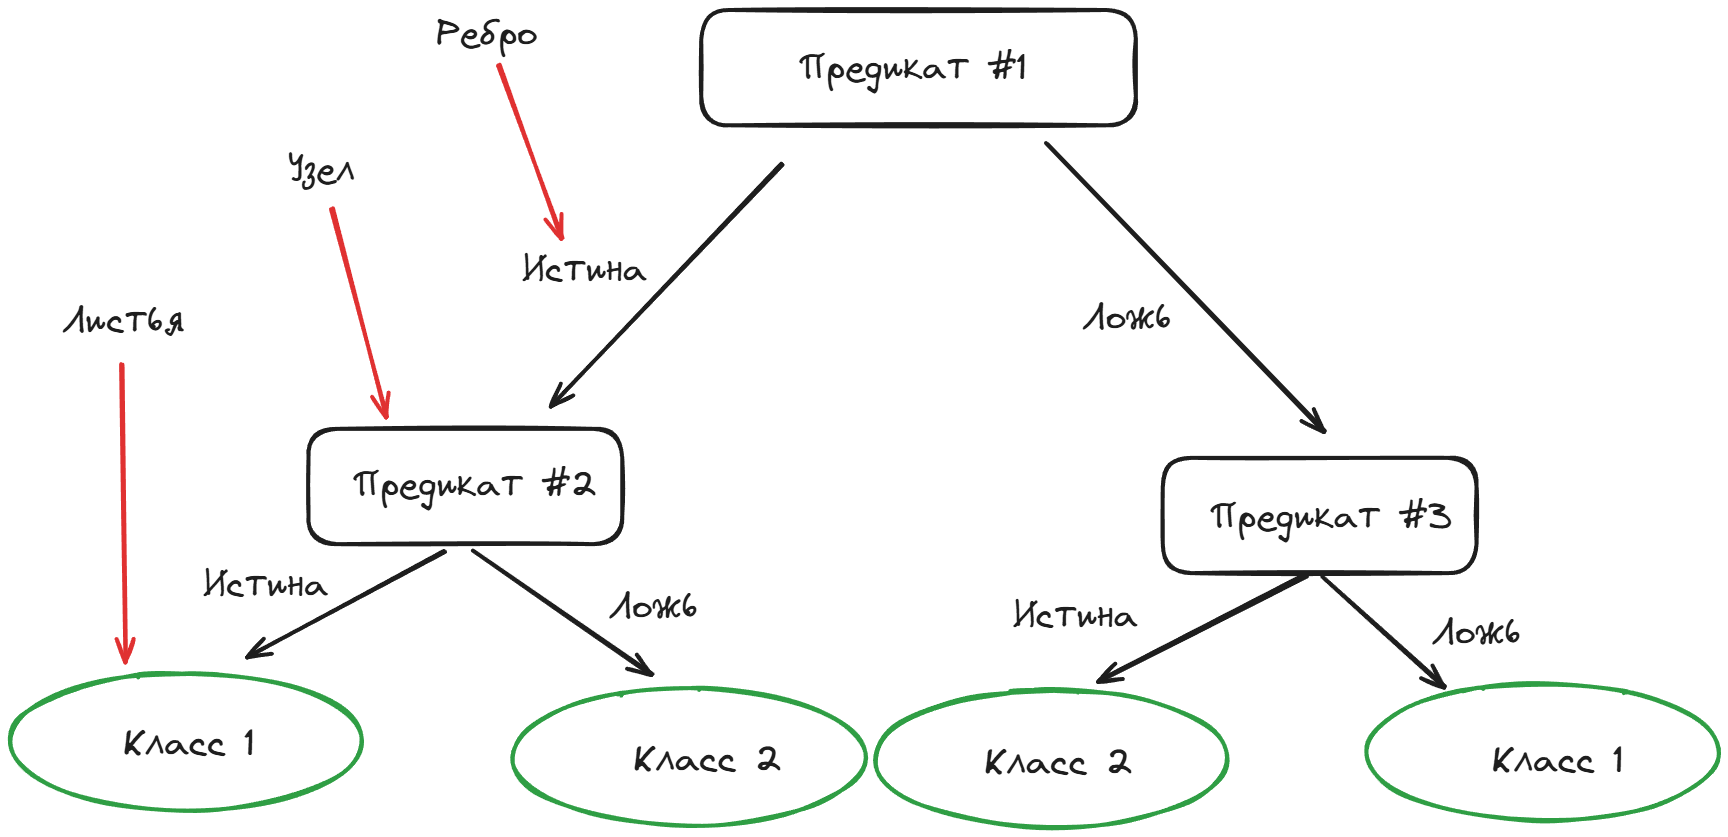
\includegraphics[width=0.8\textwidth]{pic/decision.png}
                \caption{Схема алгоритма дерева решений}
            \end{figure}

            Каждое дерево в случайном лесу представляет собой независимую
            модель, построенную на случайной подвыборке данных и случайном
            подмножестве признаков. Итоговое решение для классификации
            получается голосованием, а для регрессии — усреднением предсказаний
            деревьев. \cite{forest}

            Алгоритм работает на основе ансамблевого подхода Bagging (или же
            Bootstrap Aggregating), где каждое дерево строится на уникальной
            подвыборке данных. Это помогает снизить переобучение, так как
            деревья становятся менее зависимыми друг от друга. Для классификации
            итоговое предсказание вычисляется как:

            $$
            \hat{y} = \text{mode}(T_1(x), T_2(x), \dots, T_N(x)), \eqno(12)
            $$
            где: $T_i(x)$ — предсказание $i$-го дерева для объекта $x$,
            $\text{mode}$ — функция, возвращающая наиболее частое значение.

            Для регрессии используется усреднение предсказаний всех деревьев:

            $$\hat{y} = \frac{1}{N} \sum_{i=1}^{N} T_i(x). \eqno(13)$$

            Случайный лес строится по следующему алгоритму:

            \begin{enumerate}
                \item Создание подвыборок данных: Каждое дерево строится на
                основе случайной подвыборки данных $S_i$, полученной методом
                бутстрепа из исходного набора $S$. Размер каждой подвыборки
                равен $|S|$, но элементы могут повторяться.

                $$S_i = \{x_{i1}, x_{i2}, \dots, x_{im}\}, \quad x_{ij} \in S.$$

                \item Формирование случайного подмножества признаков: на каждом
                узле дерева выбирается случайное подмножество признаков размером
                $k$, где $k < d$ ($d$ — общее число признаков). Лучший признак
                для разбиения узла выбирается только из этого подмножества.

                \item Построение деревьев решений: каждое дерево строится до
                полной глубины (без обрезки), чтобы минимизировать ошибку на
                подвыборке.

                \item Комбинирование деревьев: для классификации применяется
                голосование, для регрессии — усреднение.
            \end{enumerate}

            Случайный лес обладает рядом преимуществ, которые делают его\\
            популярным инструментом в задачах машинного обучения. Одним из
            ключевых достоинств является устойчивость к переобучению,
            достигаемая благодаря использованию случайных подвыборок данных и
            признаков при построении деревьев. Этот подход позволяет алгоритму
            сохранять высокую точность предсказаний даже на сложных наборах
            данных. Кроме того, случайный лес предоставляет возможность оценки
            важности признаков. Для этого используется метрика уменьшения
            ошибки, определяемая как \[ \text{Importance}(j) = \frac{1}{N}
            \sum_{i=1}^{N} \left( \text{Err}_{OOB} - \text{Err}_{OOB}^{(j)}
            \right), \eqno(14) \] где \( \text{Err}_{OOB} \) обозначает ошибку
            на объектах вне подвыборки, а \( \text{Err}_{OOB}^{(j)} \) — ошибку
            после случайной перестановки признака \( j \). Это делает случайный
            лес не только эффективным инструментом для предсказания, но и мощным
            средством для анализа данных.

            Однако алгоритм имеет и свои ограничения. Одной из проблем
            является сложность интерпретации результатов, особенно в случае
            работы с большим количеством деревьев. Кроме того, случайный лес
            может быть вычислительно затратным, особенно на больших наборах
            данных, что может ограничивать его применение в условиях
            ограниченных вычислительных ресурсов.

        \subsubsection{Boosting-алгоритм CatBoost}
        
            CatBoost (Categorical Boosting) — это инструмент для решения задач
            классификации и регрессии, основанный на градиентном бустинге над
            деревьями решений. Этот алгоритм был разработан компанией Яндекс с
            учётом оптимизации работы с категориальными признаками, которые
            часто встречаются в реальных данных.
            
            Градиентный бустинг в основе CatBoost заключается в построении
            ансамбля деревьев решений, где каждое последующее дерево создаётся
            для исправления ошибок предыдущих моделей (см. Рисунок 2). Алгоритм
            минимизирует функцию потерь, последовательно добавляя деревья,
            которые корректируют остатки (разницу между фактическими значениями
            и предсказаниями текущей модели). \cite{catboost} 

            \begin{figure}[H]
                \centering
                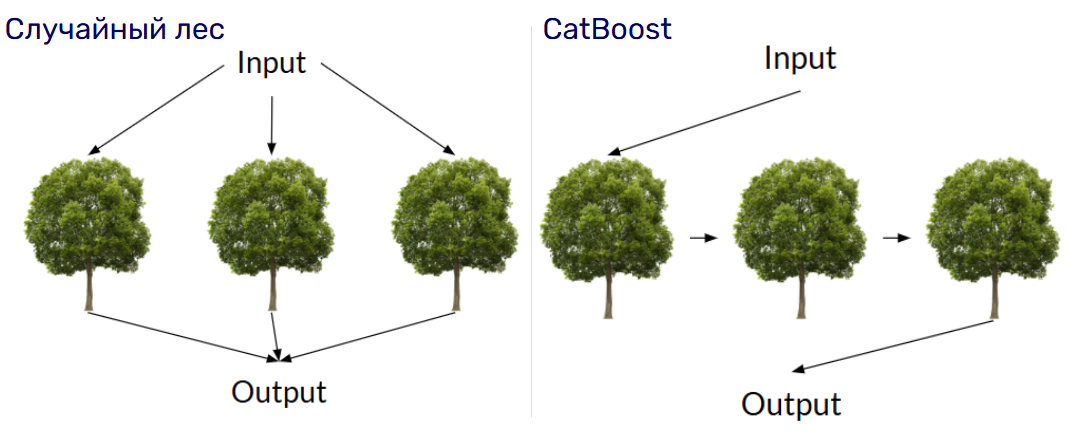
\includegraphics[width=1\textwidth]{pic/forestnboosting.png}
                \caption{Разница между случайным лесом и бустингом над деревьями решений: в первом случае деревья вычисляют значение параллельно, во втором - последовательно}
            \end{figure}

            Общая модель записывается как сумма отдельных деревьев:
            \[
            F(x) = \sum_{m=1}^M \eta \cdot h_m(x), \eqno(15)
            \]
            где \( h_m(x) \) — предсказание \( m \)-го дерева, \( \eta \) —
            коэффициент скорости обучения, а \( M \) — общее число деревьев.

            Характерной особенностью CatBoost является эффективная работа с
            категориальными признаками. Вместо простой обработки категорий с
            помощью one-hot encoding или label encoding, CatBoost использует
            метод преобразования на основе счётчиков (target encoding). Это
            позволяет учитывать распределение значений целевой переменной внутри
            категорий. Для предотвращения переобучения используется техника
            блочного разделения данных, что исключает утечку информации между
            обучением и тестированием.

            CatBoost устраняет один из ключевых недостатков градиентного
            бустинга — смещение в предсказаниях, которое возникает из-за
            некорректной инициализации или порядка построения деревьев. Это
            достигается с помощью применения "упорядоченного бустинга" (ordered
            boosting), где каждый шаг обучения модели строится на подвыборке
            данных, недоступных для текущего шага.

            Алгоритм также активно использует сжатие признаков и методы
            регуляризации, включая \( L_2 \)-регуляризацию, что делает его менее
            склонным к переобучению по сравнению с другими библиотеками, такими
            как XGBoost или LightGBM.

            CatBoost демонстрирует высокую точность предсказаний даже при работе
            с данными, содержащими большое количество категориальных признаков и
            пропущенных значений. Алгоритм требует минимальной предобработки
            данных, так как встроенные механизмы работы с категориями,
            пропусками и устойчивостью к шуму снижают необходимость в инженерии
            признаков. Более того, CatBoost обеспечивает эффективность
            вычислений благодаря использованию GPU и оптимизации
            производительности.

            Процесс минимизации ошибки модели можно выразить через задачу оптимизации:
            \[
            \min_F \sum_{i=1}^n L(y_i, F(x_i)), \eqno(16)
            \]
            где \( L(y, F(x)) \) — функция потерь, зависящая от фактического
            значения \( y \) и предсказания \( F(x) \), а \( n \) — количество
            объектов. Градиентный бустинг аппроксимирует эту функцию, добавляя
            новые деревья \( h_m(x) \), которые приближают антиградиент функции
            потерь:
            \[
            g_i^{(m)} = -\frac{\partial L(y_i, F(x_i))}{\partial F(x_i)}. \eqno(17)
            \]

        \subsubsection{Метод k-ближайших соседей}
        
            Метод $k$-ближайших соседей (k-Nearest Neighbors, k-NN) — это один
            из простейших алгоритмов машинного обучения, который используется
            для решения задач классификации и регрессии. Его суть заключается в
            том, что для нового объекта $x$ определяется $k$ ближайших объектов
            из обучающей выборки, и решение принимается на основе их значений
            (см. Рисунок 3).
            \cite{knn}

            \begin{figure}[H]
                \centering
                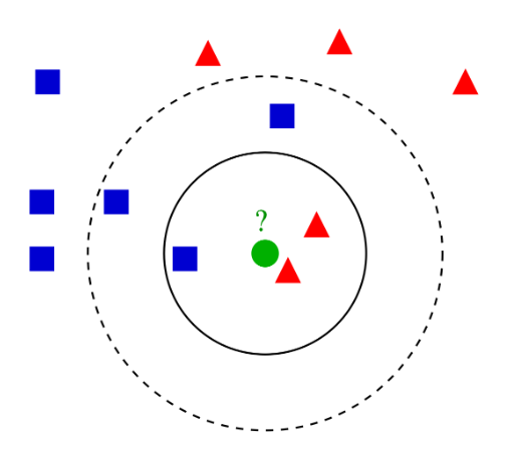
\includegraphics[width=0.7\textwidth]{pic/knn.png}
                \caption{Схема метода k-ближайших соседей}
            \end{figure}

            Для классификации метка класса нового объекта определяется по
            классу, наиболее часто встречающемуся среди $k$-ближайших соседей.
            Формально, метка $\hat{y}$ для объекта $x$ задаётся следующим
            образом:

            $$\hat{y} = \text{argmax}_c \sum_{i \in N_k(x)} \delta(y_i, c),
            \eqno(18)$$ где $N_k(x)$ — множество $k$-ближайших объектов к $x$,
            $\delta(y_i, c)$ — индикаторная функция, равная $1$, если $y_i = c$,
            и $0$ в противном случае.

            Для регрессии используется усреднение значений целевой переменной
            $y$ соседей:

            $$\hat{y} = \frac{1}{k} \sum_{i \in N_k(x)} y_i. \eqno(19)$$

            Определение расстояния между объектами осуществляется с помощью
            метрики рассчета расстояния. Выбор метрики расстояния между
            объектами играет ключевую роль в работе метода $k$-ближайших
            соседей. Наиболее популярными являются:

            \begin{enumerate}
                \item Евклидово расстояние: $$d(x, x') = \sqrt{\sum_{j=1}^d (x_j
                - x'_j)^2}, \eqno(20)$$ где $d$ — размерность пространства признаков.
                \item Манхэттенское расстояние: $$d(x, x') = \sum_{j=1}^d |x_j -
                x'_j|. \eqno(21)$$
                \item Косинусное расстояние: \[ d(x, x') = 1 -
                    \frac{\sum_{j=1}^d x_j x'_j}{\sqrt{\sum_{j=1}^d x_j^2} \cdot
                    \sqrt{\sum_{j=1}^d {x'_j}^2}}. \eqno(22)\]
            \end{enumerate}

            Евклидово расстояние является наиболее интуитивно понятной метрикой
            и работает хорошо, когда данные имеют линейную структуру и признаки
            измеряются в одинаковых единицах. Оно эффективно в задачах, где
            важно учитывать абсолютные различия между значениями признаков,
            например, в случаях с непрерывными числовыми признаками, которые
            могут быть близкими по масштабу. Однако Евклидово расстояние может
            плохо работать с разреженными данными или данными, где признаки
            имеют разную шкалу, так как большие различия в масштабе признаков
            могут сильно влиять на итоговое расстояние.

            Манхэттэнское расстояние, в отличие от Евклидова, хорошо работает в
            ситуациях, когда данные состоят из признаков, которые могут быть
            независимыми и числовыми, но не обязательно измеряются в одинаковых
            единицах. Оно полезно, например, для данных, где важно учитывать
            только отличия в отдельных признаках, а не в их комбинациях.
            Манхэттэнское расстояние подходит для задач, в которых ключевыми
            являются линейные различия, но без учета возможных ''диагональных''
            расстояний между точками. Эта метрика часто используется в задачах с
            разреженными или категориальными данными.

            Косинусное расстояние наиболее эффективно в контексте данных, где
            важно не абсолютное расстояние между объектами, а их взаимная
            направленность или угол между векторами признаков. Это делает
            косинусное расстояние идеальным для работы с текстовыми данными
            (например, при анализе документов или векторизации текстов), где два
            документа могут быть схожи по смыслу, но отличаться по длине. Эта
            метрика предпочтительна для текстовых классификаций или
            рекомендаций, где важна степень схожести в контексте общей структуры
            данных, а не в абсолютных значениях признаков.

            Для метода k ближайших соседей выбор метрики расстояния зависит от
            природы данных. Если данные являются числовыми и имеют
            нормализованные или схожие шкалы, то Евклидово расстояние обычно
            работает лучше, так как оно эффективно измеряет абсолютные различия.
            Для разреженных или категориальных данных, где важны отдельные
            различия в признаках, более подходящей может быть Манхэттэнская
            метрика. Косинусное расстояние предпочтительно, если данные
            представляют собой текстовые векторизованные представления, где
            важен не общий масштаб, а взаимная ориентация вектора признаков.
            Выбор метрики должен основываться на специфике задачи и типе данных,
            и, соответственно, каждая из метрик имеет свои преимущества в
            различных контекстах, влияя на точность и интерпретируемость
            результатов метода kNN.

    \subsection{Алгоритмы компьютерного зрения}

        \subsubsection{ResNet34}

            ResNet34 (Residual Network с 34 слоями) — это одна из архитектур
            глубоких сверточных нейронных сетей, разработанная для эффективного
            обучения глубоких моделей. Основной особенностью ResNet является
            использование так называемых остаточных блоков (residual blocks),
            которые решают проблему деградации качества обучения с увеличением
            глубины сети. Этот подход делает ResNet34 особенно эффективным для
            задач классификации, в том числе для анализа временных рядов,
            преобразованных в изображения (например, спектрограммы).
            \cite{resnet}

            Главной инновацией ResNet34 является введение остаточных соединений,
            которые позволяют передавать информацию напрямую через слои, минуя
            основной поток вычислений. Это достигается за счёт добавления
            входного сигнала \( x \) к выходу некоторого нелинейного
            преобразования \( F(x) \) (см. Рисунок 4).

            \begin{figure}[H]
                \centering
                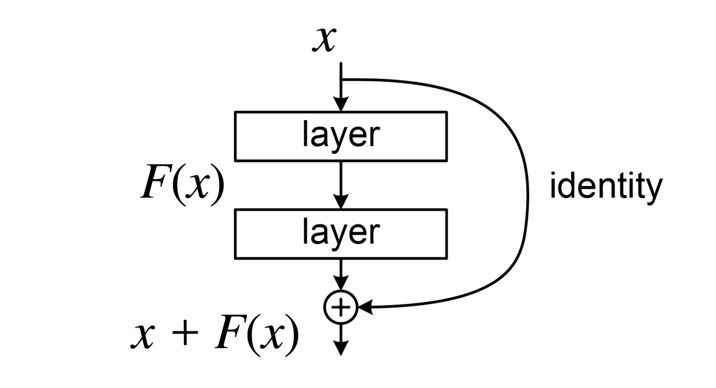
\includegraphics[width=0.7\textwidth]{pic/resblock.png}
                \caption{Особенность ResNet сети "--- Residual block}
            \end{figure}

            Математически это можно представить как:

            \[
            y = F(x) + x, \eqno(23)
            \]

            где \( F(x) \) — это результат применения свёрток, нелинейных
            функций активации и нормализации. Остаточные соединения упрощают
            обучение, так как градиенты эффективно проходят через сеть даже при
            её значительной глубине, уменьшая риск исчезающих градиентов.

            ResNet34 состоит из 34 слоев, включая свёрточные, нормализационные и
            полносвязные слои. В архитектуре предусмотрено использование
            остаточных блоков на разных уровнях, что позволяет модели обучать
            как низкоуровневые, так и высокоуровневые признаки.

            В задачах классификации временных рядов ResNet34 применяется не
            напрямую к исходным данным, а к их визуальным представлениям, таким
            как спектрограммы. Это связано с тем, что спектрограммы содержат
            временную и частотную информацию, что делает их подходящим входом
            для сверточных нейронных сетей. Использование ResNet34 в таких
            задачах позволяет:

            \begin{enumerate}
                \item Извлекать пространственные и частотные паттерны, которые
                важны для классификации временных рядов.
                \item Эффективно использовать остаточные соединения для обучения
                глубоких признаков.
                \item Уменьшить риск переобучения даже при небольшом количестве
                данных благодаря мощной регуляризации и архитектурным
                особенностям.
            \end{enumerate}

            Одним из ключевых преимуществ ResNet34 является её способность
            обучаться на больших глубинах без ухудшения производительности. Это
            делает её подходящей для сложных задач с большим количеством данных.
            Кроме того, ResNet34 демонстрирует высокую обобщающую способность,
            что особенно важно для задач классификации временных рядов, где
            данные могут быть зашумлёнными или иметь сложные зависимости.

            Однако использование ResNet34 требует значительных вычислительных
            ресурсов, что может быть ограничением для применения на устройствах
            с низкой вычислительной мощностью. Кроме того, для достижения
            оптимальной производительности требуется тщательная настройка
            гиперпараметров, включая выбор архитектурных модификаций и методов
            регуляризации.

            Благодаря своей архитектуре с остаточными соединениями и способности
            эффективно обучаться на глубоких сетях, ResNet34 становится одним из
            наиболее популярных выборов для задач классификации, где требуется
            извлечение сложных пространственных и временных паттернов. В
            контексте дипломной работы ResNet34 был использован для
            классификации спектрограмм, что позволило извлечь ключевые признаки,
            связанные с присутствием или отсутствием аврорального километрового
            радиоизлучения.

        \subsubsection{Xception}
        
            Xception (Extreme Inception) — это архитектура глубоких сверточных
            нейронных сетей, предложенная Франсуа Шолле, которая является
            развитием идей, заложенных в архитектуре Inception. Основной
            особенностью Xception является использование глубинных (separable)
            сверточных операций вместо стандартных сверточных слоев. Это делает
            модель более эффективной и вычислительно оптимизированной, сохраняя
            высокую способность к извлечению признаков. \cite{xception}
        
            Xception основывается на предположении, что пространственные и
            канальные зависимости в данных можно разъединить и обрабатывать
            независимо. В классических сверточных слоях фильтры одновременно
            анализируют пространственные и канальные связи. В Xception эти два
            процесса разделены (см. Рисунок 5):
            
                \begin{enumerate}
                    \item Глубинная свёртка (depthwise convolution): каждая
                    свёртка применяется к отдельному каналу данных, что
                    позволяет обрабатывать пространственную информацию
                    независимо.
                    \item Точечная свёртка (pointwise convolution): применяется
                    \(1 \times 1\)-свёртка, которая агрегирует информацию из
                    всех каналов.
                \end{enumerate}

            \begin{figure}[H]
                \centering
                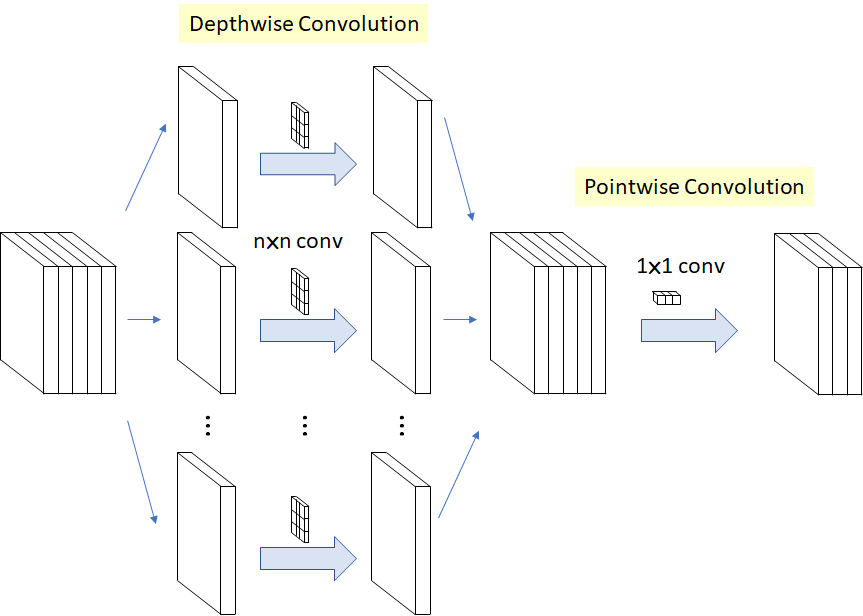
\includegraphics[width=0.8\textwidth]{pic/xception.png}
                \caption{Визуализация глубинной и точечной свертки}
            \end{figure}

            Такой подход можно выразить математически. Пусть входной тензор
            имеет размерность \(H \times W \times C_{\text{in}}\), где \(H\) и
            \(W\) — пространственные размеры, а \(C_{\text{in}}\) — количество
            входных каналов. Глубинная свёртка вычисляется как:
        
            \[
            \text{DepthwiseConv}(x)_{i,j,k} = \sum_{m,n} x_{i+m, j+n, k} \cdot w_{m,n,k}, \eqno(24)
            \]
            
            где \(w_{m,n,k}\) — веса фильтра для каждого канала. После этого
            точечная свёртка объединяет результаты:
            
            \[
            \text{PointwiseConv}(y)_{i,j,c} = \sum_{k} y_{i,j,k} \cdot w_{k,c}. \eqno(25)
            \]
        
            Этот процесс уменьшает вычислительную сложность с \\ \(O(H \cdot W
            \cdot C_{\text{in}} \cdot C_{\text{out}} \cdot K^2)\) до \(O(H \cdot
            W \cdot (C_{\text{in}} \cdot K^2 + C_{\text{in}} \cdot
            C_{\text{out}}))\), где \(K\) — размер ядра свёртки.
        
        
            Для задач классификации временных рядов Xception применяется к их
            визуальным представлениям, таким как спектрограммы. Это позволяет
            использовать пространственно-канальную декомпозицию для анализа
            временной и частотной информации. Xception оказывается особенно
            эффективным в таких задачах благодаря следующим свойствам:
            
            \begin{enumerate}
                \item Разделение пространственных и канальных свёрток позволяет
                лучше адаптироваться к сложной структуре спектрограмм.
                \item Небольшое количество параметров модели делает её более
                подходящей для обучения на ограниченных ресурсах.
                \item Глубокие слои с эффективным извлечением признаков
                обеспечивают высокую точность даже на сложных наборах данных.
            \end{enumerate}
            
            Ключевым преимуществом Xception является её способность\\
            обрабатывать данные с высокой вычислительной эффективностью,
            сохраняя точность предсказаний. Модель хорошо справляется с
            извлечением сложных пространственно-частотных признаков из
            спектрограмм, что делает её подходящей для задач анализа временных
            рядов. Однако Xception требует большого объема данных для обучения,
            так как её глубокая архитектура может склоняться к переобучению на
            малых выборках. 
            
            Xception демонстрирует свою эффективность в задачах классификации
            временных рядов, где требуется анализ сложных структур данных. В
            контексте дипломной работы архитектура Xception использовалась для
            обработки спектрограмм, что позволило извлечь детализированные
            признаки, отражающие как временные, так и частотные аспекты сигнала.
            Модель доказала свою эффективность благодаря гибкости и
            вычислительной оптимизации, обеспечив высокую точность в задаче
            детекции аврорального километрового радиоизлучения.

        \subsubsection{ViT}

            Vision Transformer (ViT) представляет собой архитектуру глубокого
            обучения, впервые предложенную для обработки изображений, основанную
            на механизме самовнимания (self-attention). ViT отличается от
            классических сверточных сетей (CNN) тем, что не использует свёртки
            для извлечения признаков, а применяет трансформеры, изначально
            разработанные для задач обработки естественного языка. \cite{vit}
            Это делает ViT мощным инструментом для анализа структурированных
            данных, таких как спектрограммы временных рядов (см. Рисунок 6).
            
            \begin{figure}[H]
                \centering
                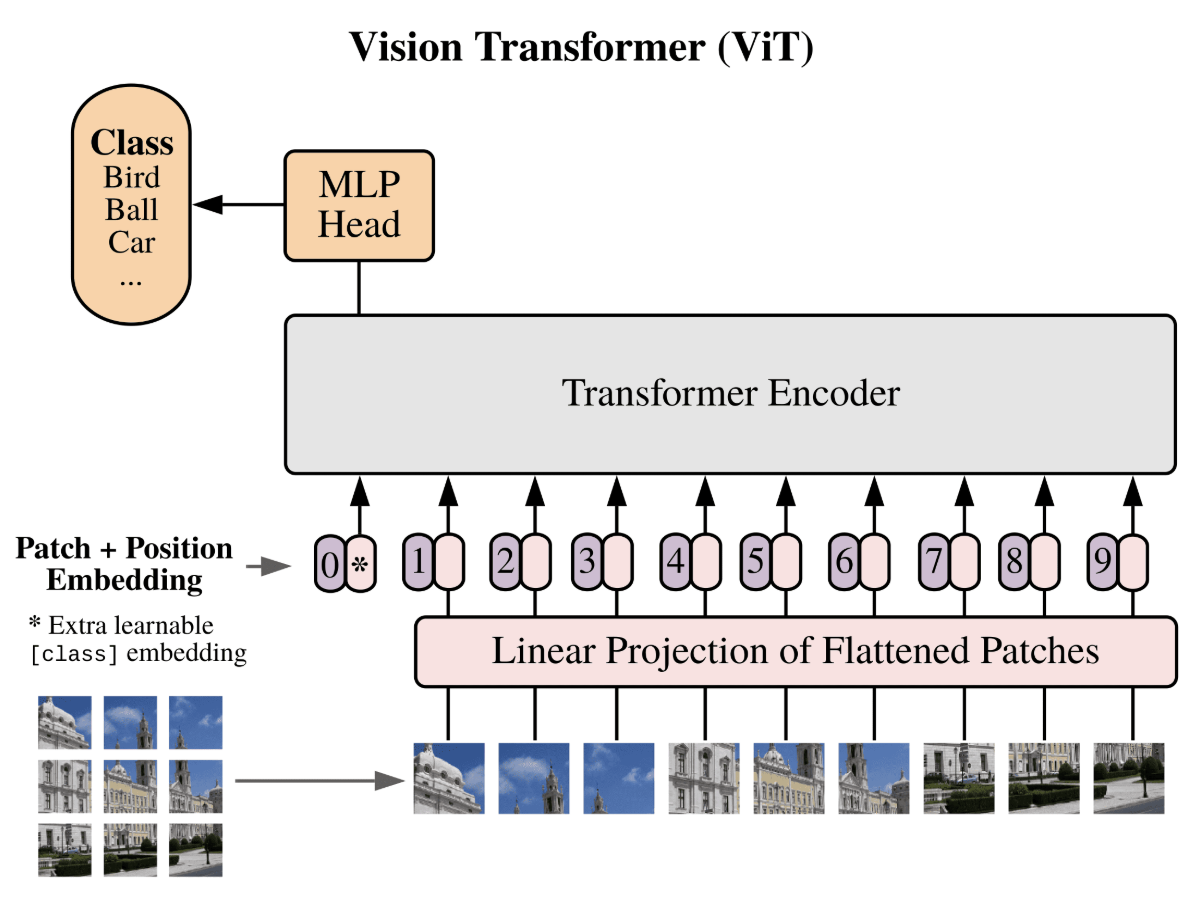
\includegraphics[width=0.8\textwidth]{pic/vit.png}
                \caption{Архитектура Vision Transformer \cite{firstvit}}
            \end{figure}

            В основе механизма самовнимания, используемого в Vision Transformer
            (ViT), лежит определение матриц запросов (\(Q\)), ключей (\(K\)) и
            значений (\(V\)). Эти матрицы определяют, как различные части
            данных, такие как патчи изображения или временные интервалы в
            спектрограммах, взаимодействуют друг с другом. Для каждого входного
            патча \(x_p\) создаются три линейных преобразования, которые
            формируют его представление как запрос (\(q_p\)), ключ (\(k_p\)) и
            значение (\(v_p\)). Математически это выражается через линейные
            операции:
            \[
            q_p = W_q \cdot x_p,\quad k_p = W_k \cdot x_p,\quad v_p = W_v \cdot x_p, \eqno(26)
            \]
            где \(W_q\), \(W_k\), \(W_v\) — обучаемые матрицы весов, а \(x_p\) —
            исходное представление патча. 
        
            Итоговое представление патча формируется как взвешенная сумма
            значений \(v_j\), где веса определяются матрицей внимания. Такой
            подход позволяет модели выделять наиболее значимые связи между
            различными частями данных, что делает ViT особенно эффективным в
            анализе структурированных данных, таких как изображения или
            спектрограммы временных рядов.
            
            ViT работает с изображениями или другими матрицами данных следующим
            образом:
            
            \begin{enumerate}
                \item Изображение в ViT сначала разбивается на несколько
                маленьких равных прямоугольных блоков (патчей), обычно размером
                \( 16 \times 16 \) пикселей или \( 32 \times 32 \) пикселей, в
                зависимости от конфигурации. Каждый такой патч \( x_p \)
                преобразуется в одномерный вектор с помощью операции
                ''плоского'' преобразования (flattening), где все значения
                пикселей патча, например, в случае RGB изображения, будут
                записаны в длинный вектор. Размер этого вектора будет зависеть
                от размеров патча и числа цветовых каналов (например, для
                RGB-изображения с патчами \( 16 \times 16 \) это будет вектор
                размером \( 16 \times 16 \times 3 = 768 \)).
            
                Таким образом, \( x_p \) — это одномерный вектор, представляющий
                собой информацию о конкретном патче изображения или фрагменте
                данных (в случае анализа временных рядов, например, это может
                быть вектор, описывающий фрагмент временного ряда).

                \item Каждый патч преобразуется с помощью линейного слоя, формируя
                векторное представление \(z_p\), где \(p\) — индекс патча:
                \[
                z_p = W_p \cdot \text{vec}(x_p) + b_p, \eqno(27)
                \]
                где \(W_p\) — матрица весов, \(\text{vec}\) — операция
                векторизации, а \(x_p\) представляет собой векторное
                представление патча изображения.

                \item К каждому вектору добавляется позиционная информация, чтобы
                модель могла учитывать относительное расположение патчей:
                
                \[
                    z_p^{(0)} = z_p + \text{pos}_p. \eqno(28)
                \]

                Поскольку в стандартных трансформерах отсутствует явная
                информация о порядке входных элементов (например, о
                пространственном расположении пикселей в изображении),
                позиционное кодирование добавляется к представлениям патчей,
                чтобы предоставить информацию о пространственной или временной
                позиции каждого патча в исходном изображении. Позиционное
                кодирование \( pos_p \) для каждого патча \( p \) — это вектор
                фиксированного размера, который добавляется к соответствующему
                вектору патча. Это позволяет модели учитывать порядок и
                пространственные отношения между патчами. В ViT позиционные
                кодировки обычно создаются с использованием синусоидальных
                функций или обучаемых векторов.

                \item Представления патчей обрабатываются через трансформер, который
                вычисляет взвешенные связи между всеми патчами, определяя их
                взаимное влияние:

                \[
                    \text{Attention}(Q, K, V) = \text{softmax}\left(\frac{QK^\top}{\sqrt{d_k}}\right)V, \eqno(29)
                \]        
                
                где \(Q, K, V\) — матрицы запросов, ключей и значений, \(d_k\) —
                размерность представлений, а softmax "--- функция, которая
                преобразует вектор чисел в вероятностное распределение, где
                сумма всех элементов равна \(1\). Для заданного вектора \(z =
                [z_1, z_2, \ldots, z_n]\), функция softmax вычисляется следующим
                образом:

                \[
                \text{softmax}(z_i) = \frac{\exp(z_i)}{\sum_{j=1}^n \exp(z_j)}, \eqno(30)
                \]

                где: \(z_i\) — \(i\)-й элемент входного вектора, \(\exp(z_i)\) —
                экспонента от \(z_i\), т.е. \(e^{z_i}\), где \(e\) — основание
                натурального логарифма, \(\sum_{j=1}^n \exp(z_j)\) — нормирующий
                коэффициент, равный сумме всех экспонент элементов вектора.

                \item После нескольких слоев самовнимания и нормализации итоговое
                представление патчей передается в полносвязный слой, чтобы получить
                предсказание.
            \end{enumerate}

            ViT был адаптирован для анализа временных рядов путём преобразования
            их в спектрограммы, которые затем рассматриваются как изображения.
            Основное преимущество ViT в этой задаче — его способность
            моделировать глобальные зависимости между разными частями данных,
            что особенно важно для временных рядов с комплексными взаимосвязями.
            
            При обработке спектрограмм временных рядов Vision Transformer (ViT)
            демонстрирует ряд ключевых свойств. Во-первых, механизм самовнимания
            позволяет учитывать взаимосвязи между удалёнными регионами
            спектрограммы, что обеспечивает глубокое понимание глобального
            контекста и особенно важно для временных рядов с долгосрочной
            зависимостью. Во-вторых, ViT отличается гибкостью: отказ от
            использования свёрток предоставляет модели больше свободы в
            обработке данных с нетривиальными структурными особенностями,
            позволяя эффективно адаптироваться к различным типам спектрограмм.
            Наконец, ViT демонстрирует высокую производительность на больших
            наборах данных благодаря своей архитектуре, однако может уступать
            классическим сверточным нейронным сетям (CNN) на небольших выборках
            из-за высокой сложности и большого числа параметров, что требует
            значительных объемов данных для обучения.
            
            ViT обладает выдающейся способностью извлекать\\ детализированные
            признаки и анализировать взаимосвязи между частями данных. Однако
            одной из сложностей является необходимость большого объема данных
            для обучения, так как трансформеры имеют тенденцию к переобучению на
            малых выборках. Кроме того, разделение данных на патчи может
            приводить к потере мелкомасштабной информации, особенно если размер
            патча выбран неудачно.
            
            ViT представляет собой инновационный подход к обработке временных
            рядов, предлагая эффективное использование спектрограмм для анализа.
            В рамках дипломной работы использование ViT позволило исследовать
            глобальные зависимости в данных, что является важным для
            классификации сложных временных сигналов, таких как авроральное
            километровое радиоизлучение. Модель показала высокую точность и
            способность к генерализации, что подчёркивает её потенциал в задачах
            анализа временных рядов.

    \subsection{Метрики оценки качества обучения}

        В задачах классификации, включая задачи обнаружения аномалий в
        мультивариативных временных рядах, важно правильно оценивать качество
        работы модели. Одним из ключевых инструментов для этого являются
        метрики, которые позволяют понять, насколько точно и правильно модель
        классифицирует данные. В этой главе рассмотрены две важные метрики —
        Confusion Matrix и F1-score которые активно используются в практике
        машинного обучения для оценки эффективности классификаторов.
        \cite{scores}, \cite{mat}
        
        Матрица ошибок или Confusion Matrix представляет собой таблицу, которая
        отображает количество правильных и неправильных предсказаний модели в
        различных категориях. Она показывает, как алгоритм классификации
        ошибается в отношении каждой из классов. Матрица состоит из следующих
        элементов:
        
        \begin{figure}[H]
            \centering
            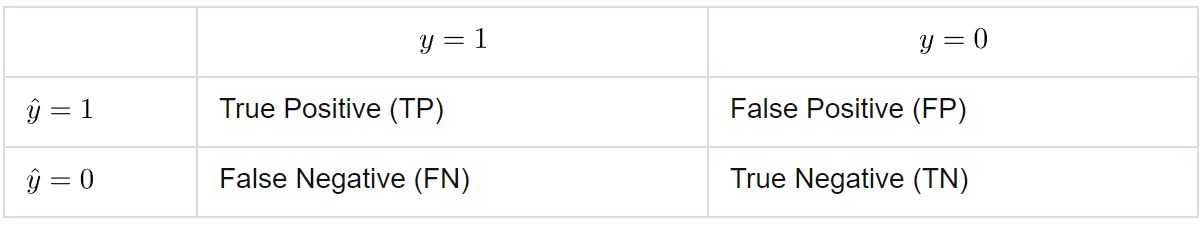
\includegraphics[width=0.9\textwidth]{pic/matrix.png}
            \caption{Матрица ошибок}
        \end{figure}
        
        Где:

        \begin{enumerate}
            \item \( TP \) (True Positive) — количество истинных положительных
            предсказаний (модель правильно предсказала положительный класс).
            \item \( TN \) (True Negative) — количество истинных отрицательных
            предсказаний (модель правильно предсказала отрицательный класс).
            \item \( FP \) (False Positive) — количество ложных положительных
            предсказаний (модель ошибочно предсказала положительный класс, когда
            на самом деле класс был отрицательным).
            \item \( FN \) (False Negative) — количество ложных отрицательных
            предсказаний (модель ошибочно предсказала отрицательный класс, когда
            на самом деле класс был положительным).
        \end{enumerate}
        
        С помощью матрицы ошибок можно вычислить несколько ключевых метрик,
        таких как точность, полнота, F1-score, которые помогут оценить работу
        модели. Например:
        
        Точность (Accuracy) — доля правильных предсказаний, вычисляется как:
        
        \[
        \text{Accuracy} = \frac{TP + TN}{TP + TN + FP + FN}. \eqno(31)
        \]
        
        Полнота (Recall) — доля правильных положительных предсказаний среди всех
        реально положительных случаев:
        
        \[
        \text{Recall} = \frac{TP}{TP + FN}. \eqno(32)
        \]
        
        Точность (Precision) — доля правильных положительных предсказаний среди
        всех предсказанных положительных случаев:
        
        \[
        \text{Precision} = \frac{TP}{TP + FP}. \eqno(33)
        \]
        
        F1-score является гармоническим средним между точностью (Precision) и
        полнотой (Recall). Эта метрика особенно полезна, когда важно
        сбалансировать точность и полноту, и когда набор данных может быть
        несимметричным, то есть один класс значительно преобладает над другим.
        
        F1-score вычисляется по следующей формуле:
        
        \[
        F1 = 2 \times \frac{\text{Precision} \times \text{Recall}}{\text{Precision} + \text{Recall}}. \eqno(34)
        \]
        
        F1-score принимает значения от 0 до 1, где значение 1 означает идеальное
        качество модели (все предсказания правильные), а значение 0 указывает на
        полное отсутствие предсказаний. F1-score особенно полезен в тех случаях,
        когда важно учитывать как ложные отрицательные, так и ложные
        положительные предсказания, а не просто количество правильных
        предсказаний.
        
        В задачах обнаружения аномалий матрица ошибок и F1-score позволяют
        осуществить оценку эффективности модели. Аномалии, как правило,
        составляют меньшинство в наборе данных, что делает задачу
        несимметричной. В таких случаях модель может показывать высокую точность
        за счет предсказания большинства примеров как нормальных, но при этом
        пропускать аномалии. В таких ситуациях F1-score является более
        информативной метрикой, так как она учитывает и ложные отрицательные, и
        ложные положительные предсказания, помогая обеспечить более
        сбалансированную оценку работы модели.
        
        Для задач с большими дисбалансами в данных (когда один класс значительно
        преобладает над другим) F1-score может быть особенно полезным, так как
        простое использование точности может не давать полной картины
        эффективности модели.

\section{Практическая часть}

    В открытом доступе существует крайне ограниченное количество реальных данных
    логирования параметров атак на компьютерные системы. Это объясняется как
    соображениями конфиденциальности, так и сложностью сбора и предоставления
    таких данных для публичного анализа. Использование синтетических данных для
    моделирования сетевых атак, хотя и является распространённой практикой,
    имеет свои ограничения. Синтетические данные часто не отражают всех важных
    характеристик и параметров реальных атак, что снижает их ценность для
    тестирования и анализа алгоритмов машинного обучения в условиях,
    приближенных к реальным.

    В связи с этим было принято решение исследовать методы машинного обучения на
    примерах реальных задач, которые, хотя и не относятся напрямую к области
    компьютерной безопасности, обладают схожими характеристиками по структуре
    данных и сложности анализа. Такой подход позволяет избежать недостатков,
    связанных с использованием синтетических данных, и сосредоточиться на
    разработке методик, применимых к широкому спектру задач.

    Полученная в ходе данного исследования методика обработки данных и
    применения алгоритмов машинного обучения может быть адаптирована и
    использована для анализа данных, относящихся к компьютерной безопасности.
    Это открывает возможности для разработки более точных и надёжных решений,
    применяемых в задачах обнаружения аномалий и предотвращения кибератак.

    Цель данного практического исследования состоит в поиске, изучении и
    рассмотрении возможных способов качественного обнаружения аномалий в
    мультивариативном временном ряду на примере задачи детекции аврорального
    километрового радиоизлучения. Данная задача имеет важное значение для
    исследований в области космической физики, поскольку авроральное
    радиоизлучение связано с электромагнитными процессами в магнитосфере Земли,
    влияющими на космическую погоду и работу спутниковых систем. Актуальность
    задачи обусловлена растущей необходимостью мониторинга и прогнозирования
    таких явлений для минимизации рисков, связанных с влиянием космической
    погоды на телекоммуникации и навигацию.

    \subsection{Описание исходного набора данных}

        Данные были получены с официального сайта ''NASA's Space Physics Data
        Facility (SPDF)''. NASA's Space Physics Data Facility (SPDF)
        представляет собой онлайн-ресурс, предоставляющий доступ к обширному
        набору данных, связанных с физикой космоса и исследованиями
        солнечно-земных взаимодействий. Этот ресурс является хранилищем научных
        данных, собранных с помощью спутников NASA, международных космических
        миссий и наземных наблюдений. На сайте SPDF можно найти временные ряды,
        спектры, данные о магнитных полях, электрических полях, частицах и
        электромагнитных волнах в различных космических средах, таких как
        межпланетное пространство, магнитосфера Земли и солнечный ветер.
        Доступные данные включают как исторические записи, так и текущие
        результаты миссий, таких как WIND, THEMIS и MAVEN. Ресурс активно
        используется исследователями для изучения космической погоды, анализа
        авроральных процессов и других явлений, что делает его важным
        инструментом для работы в области астрофизики и космических технологий.
        \cite{space}

        В данной работе в качестве мультивариативного временного ряда
        использовались данные спутника GGS WIND, которые представляют собой
        значения напряженности электрического поля для частот от 20 кГц до 13825
        кГц, измеряемые раз в минуту на протяжении 18720 минут. Измерения были
        зафиксированы в период времени с 1 июля 2020 года в 00:00:30 по 13 июля
        2020 года в 23:59:30. Каждой частоте в диапазоне с шагом 4 кГц
        соответствовал отдельный временной ряд, фиксирующий напряженность
        электрического поля в конкретный момент времени.

        Данные на сайте NASA's Space Physics Data Facility (SPDF) обычно
        хранятся в формате Common Data Format (CDF). Этот формат оптимизирован
        для хранения научных данных, таких как временные ряды, спектры или
        многомерные массивы, и поддерживает метаданные, описывающие структуру и
        содержание файла. Файлы CDF содержат переменные, которые могут быть
        скалярными (одномерными) или многомерными массивами. Каждая переменная
        сопровождается атрибутами, описывающими единицы измерения, источник
        данных и другие характеристики.

        Данные для исследования содержались в 13 файлах формата cdf. Структура
        данных в каждом файле CDF выглядит следующим образом:

        \begin{minted}[fontsize=\footnotesize]{text}
            E_VOLTAGE_RAD1: CDF_REAL4 [1440, 256]
            E_VOLTAGE_RAD2: CDF_REAL4 [1440, 256]
            E_VOLTAGE_TNR: CDF_REAL4 [1440, 96]
            Epoch: CDF_EPOCH [1440]
            Epoch2: CDF_EPOCH [1]
            Frequency_RAD1: CDF_INT2 [256] NRV
            Frequency_RAD2: CDF_INT2 [256] NRV
            Frequency_TNR: CDF_REAL4 [96] NRV
            Minimum_voltage_RAD1: CDF_REAL4 [1, 256]
            Minimum_voltage_RAD2: CDF_REAL4 [1, 256]
            Minimum_voltage_TNR: CDF_REAL4 [1, 96]
        \end{minted}

        В данном случае:
        
        \begin{enumerate}
            \item E_VOLTAGE_RAD1 "--- эта переменная содержит значения
            электрического напряжения, зарегистрированные инструментом RAD1
            (Radio Receiver Band 1) за каждый момент времени. Первая размерность
            (1440) соответствует количеству временных отсчётов в течение дня, а
            вторая (256) — количеству частотных каналов. Данные представлены в
            формате CDF_REAL4, что означает числа с плавающей точкой (4 байта).
            Они используются для анализа сигналов в определённом диапазоне
            частот;
            \item E_VOLTAGE_RAD2 "--- аналогично переменной E_VOLTAGE_RAD1, эта
            переменная содержит данные о напряжении, зарегистрированном
            инструментом RAD2 (Radio Receiver Band 2), работающем в другом
            диапазоне частот. Формат и структура совпадают с E_VOLTAGE_RAD1;
            \item E_VOLTAGE_TNR "--- эта переменная представляет напряжение,
            зарегистрированное инструментом TNR (Thermal Noise Receiver),
            который фиксирует тепловой шум. Размерность массива отличается: 96
            частотных каналов и 1440 временных отсчётов. Инструмент TNR
            используется для более точного анализа сигналов в нижнем диапазоне
            частот;
            \item Переменная Epoch представляет временные метки для каждого из
            1440 измерений в течение дня. Формат CDF_EPOCH используется для
            представления временных данных в формате UTC с высокой точностью,
            что позволяет сопоставить данные с глобальным временем наблюдений;
            \item Переменная Epoch2 содержит единственную временную метку,
            представляющую общее время начала записи данных или другой важный
            временной момент, относящийся ко всему файлу;
            \item Переменная Frequency_RAD1 представляет массив частотных
            каналов, соответствующих измерениям инструмента RAD1. Формат
            CDF_INT2 означает, что данные хранятся в виде 16-битных целых чисел.
            Маркер NRV (No Record Variance) указывает, что эти значения
            постоянны для всех временных отсчётов;
            \item Frequency_RAD2, аналогично Frequency_RAD1, содержит частоты
            для инструмента RAD2. Они остаются неизменными для всех временных
            меток;
            \item Переменная Frequency_TNR содержит частоты, использованные
            инструментом TNR. Данные представлены в формате CDF_REAL4 и имеют
            более низкое разрешение (96 каналов). Они также не зависят от
            временных отсчётов;
            \item Переменная Minimum_voltage_RAD1 содержит минимальные значения
            напряжения для каждого частотного канала, зарегистрированные
            инструментом RAD1. Первая размерность (1) указывает на то, что
            данные фиксированы для всех временных отсчётов;
            \item Данные Minimum_voltage_RAD2, аналогично Minimum_voltage_RAD1,\\
            отражают минимальные значения напряжения для инструмента RAD2 по
            каждому из частотных каналов;
            \item Переменная Minimum_voltage_TNR содержит минимальные значения
            напряжения для инструмента TNR. Меньшее количество частотных каналов
            (96) соответствует специфике работы этого инструмента.
        \end{enumerate}

    \subsection{Описание инструментов и библиотек программной реализации}

        В процессе выполнения данной работы использовались современные
        программные инструменты и библиотеки, которые обеспечивают высокую
        эффективность при работе с данными, машинным обучением и глубоким
        обучением. Ниже приведено краткое описание основных из них.

        Python является универсальным и широко используемым языком
        программирования, идеально подходящим для анализа данных, статистической
        обработки и машинного обучения. Его обширная экосистема библиотек делает
        его незаменимым инструментом для научных исследований. \cite{python}

        Pandas предоставляет удобный интерфейс для работы с табличными данными.
        С помощью этой библиотеки можно легко обрабатывать, фильтровать и
        агрегировать данные, а также преобразовывать их в удобные форматы, такие
        как датафреймы. Pandas использовалась для обработки данных, извлечённых
        из формата CDF, и для подготовки входных данных для машинного обучения.
        \cite{fwpandas}

        Библиотека SpacePy, а точнее её модуль pycdf, позволяет работать с
        файлами в формате Common Data Format (CDF). Данная библиотека
        использовалась для извлечения временных рядов из данных NASA и их
        последующей конвертации в датафреймы. \cite{fwspacepy}

        NumPy предоставляет средства для работы с массивами данных и числовыми
        вычислениями. Эта библиотека была использована для выполнения линейной
        алгебры, обработки многомерных массивов и подготовки данных для
        визуализации спектрограмм. \cite{fwnumpy}

        Scikit-learn — библиотека для классических методов машинного обучения.
        Она использовалась для реализации алгоритма метода k ближайших соседей
        (kNN), а также для оценки качества моделей с помощью метрик, таких как
        F1-score. \cite{fwsl}
        
        Библиотека PyTS предоставляет набор инструментов для работы с временными
        рядами, включая различные методы классификации, преобразования и
        анализа. Одним из важных для данной работы компонентов этой библиотеки
        является класс TimeSeriesForest, который представляет собой алгоритм
        классификации для временных рядов, основанный на случайных лесах. Этот
        метод предназначен для решения задач классификации, где данные
        представлены в виде временных рядов. \cite{fwpyts}
        
        CatBoost — библиотека для обучения градиентного бустинга. Она эффективно
        работает с категориальными признаками и была применена для построения
        моделей классификации временных рядов. \cite{fwcatboost}

        Pickle — стандартная библиотека Python для сериализации объектов. Она
        применялась для сохранения и загрузки обученных моделей, чтобы
        обеспечить их повторное использование без необходимости повторного
        обучения. \cite{fwpickle}

        SciPy предоставляет множество инструментов для научных вычислений.
        Модуль scipy.signal.spectrogram использовался для построения
        спектрограмм временных рядов с помощью оконного преобразования Фурье.
        \cite{fwscipy}
        
        Matplotlib — основная библиотека для построения графиков и визуализации
        данных. Seaborn — её надстройка, которая упрощает создание эстетичных и
        информативных визуализаций. \cite{fwmatplotlib} Эти библиотеки
        использовались для анализа данных, визуализации результатов и создания
        спектрограмм. \cite{fwseaborn}

        PyTorch — одна из наиболее популярных библиотек для глубокого обучения.
        Она предоставляет гибкий интерфейс для построения и обучения нейронных
        сетей. PyTorch использовалась для реализации модели ResNet34, а также
        для обучения других нейронных сетей. \cite{fwpytorch}

        Torchvision — библиотека для работы с изображениями, входящая в состав
        экосистемы PyTorch. Она предоставляет предобученные модели, включая
        ResNet34, а также инструменты для обработки изображений.
        \cite{fwtorchvision}

        Timm (PyTorch Image Models) — библиотека, предоставляющая доступ к
        большому количеству архитектур нейронных сетей для задач компьютерного
        зрения. В данном исследовании с её помощью была использована модель
        Xception. \cite{fwtimm}

        Transformers — библиотека от Hugging Face для работы с трансформерными
        архитектурами. Она предоставляет готовые реализации моделей, таких как
        ViT (Vision Transformer), которые были использованы для классификации
        временных рядов. \cite{fwtransformers}

    \subsection{Обработка набора данных}

        Авроральное километровое радиоизлучение (АКР) — это интенсивное
        природное радиоизлучение в диапазоне частот 30–800 кГц, создаваемое в
        околоземной плазме и распространяющееся от Земли. Необходимый диапазон
        частот был указан в параметре Frequency_RAD1. Так как ему соответствует
        массив E_VOLTAGE_RAD1 значений нормализованного напряжения
        электрического поля, дальнейшее исследование и обработка осуществлялось
        относительно него. Все остальные массивы данных помимо выше упомянутых и
        параметра Epoch использованы не были.
        
        С помощью библиотеки SpacePy и Pandas было осуществлено преобразование
        исходных массивов данных в более удобный формат для обработки средствами
        машинного обучения и нейросетями. Далее были вручную выделены временные
        промежутки, на которых наблюдалось АКР. Каждому моменту времени было
        сопоставлено значение, которое равнялось единице, если в этот момент
        времени наблюдалось АКР, или равнялось нулю, если в этот момент времени
        АКР не наблюдалось.

        В результате получился мультивариативный временной ряд, состоящий из 256
        временных рядов, разделенных на интервалы, где фиксировалось наличие или
        отсутствие аврорального километрового излучения (см. Рисунок 8 и 9).

        \begin{figure}[H]
            \centering
            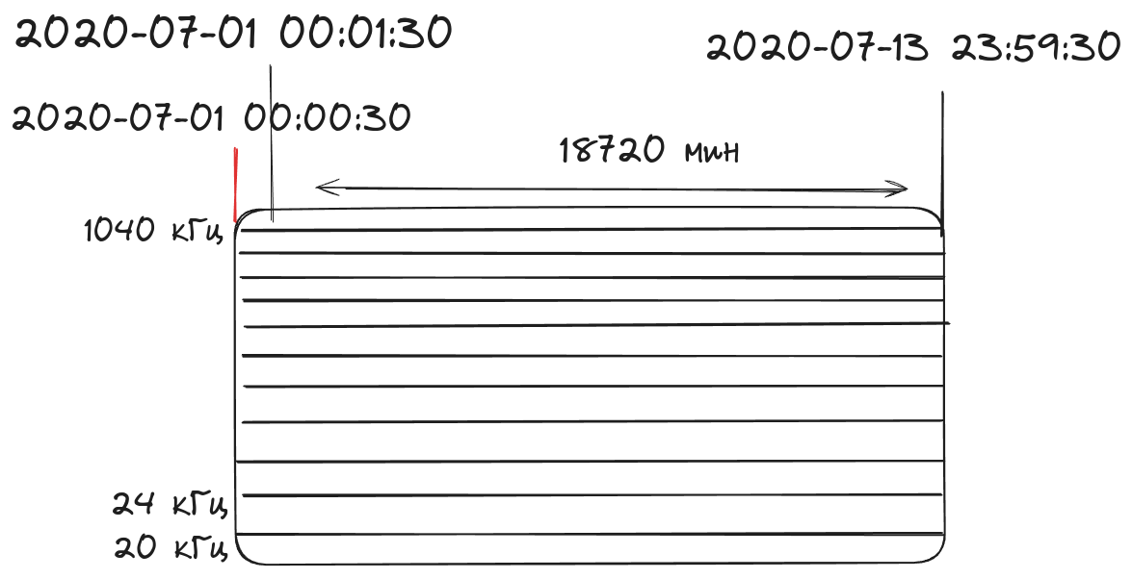
\includegraphics[width=1\textwidth]{pic/data.png}
            \caption{Схематичное изображение набора данных (в диапазоне частот от 20 кГц до 1040 кГц)}
        \end{figure}

        \begin{figure}[H]
            \centering
            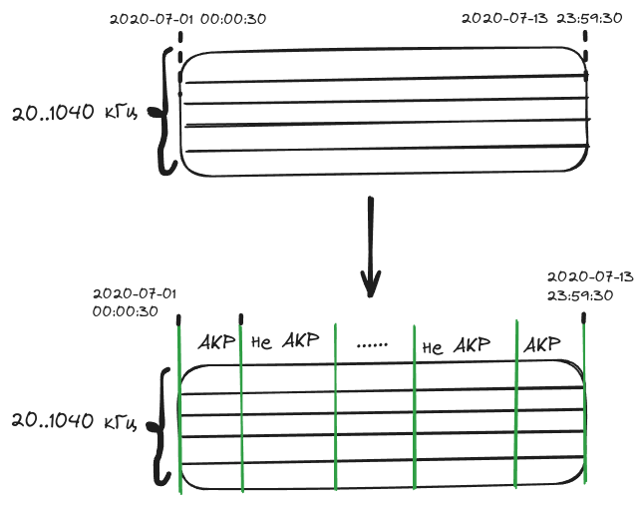
\includegraphics[width=1\textwidth]{pic/labeling.png}
            \caption{Схематичное изображение состояния набора данных после разметки}
        \end{figure}

        Так как используемые мною для классификации нейронные сети и алгоритмы
        машинного обучения предполагают одинаковую размерность всех входных
        образцов, на втором этапе обработки данных стояла задача разделения
        мультивариативного временного ряда на интервали/блоки одинаковой
        размерности.

        Для выбора оптимальной размерности были проанализированы длительности
        интервалов с АКР и интервалов без АКР. Минимальная длительность
        промежутка с АКР составила 4 минуты, максимальная — 1193 минуты.
        Минимальная длительность промежутка без АКР составила 2 минуты,
        максимальная — 2433 минуты. Было построено и визуализированно нормальное
        распределение значений длительности АКР, на основании которого
        осуществлялся выбор размерности блоков (см. Таблица 1 и Рисунок 10).

        \begin{figure}[H]
            \centering
            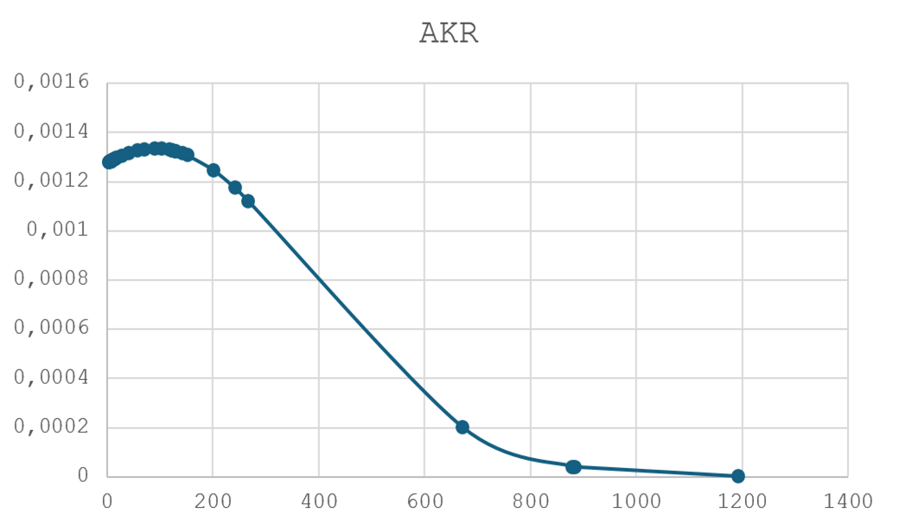
\includegraphics[width=1\textwidth]{pic/dist.png}
            \caption{Нормальное распределение значений длительности АКР. Ось X "--- значения длительности промежутков АКР, ось Y - плотность вероятности}
        \end{figure}

        \begin{table}[h]
            \centering
            \label{tab:akr_duration}
            \begin{tabular}{|c|c|c|c|c|c|}
            \hline
            \textbf{Длит-ть} & \textbf{Плотность} & \textbf{Длит-ть} & \textbf{Плотность} & \textbf{Длит-ть} & \textbf{Плотность} \\ \hline
            4    & 0.001279747  & 8    & 0.001284630  & 58   & 0.001327042  \\ \hline
            4    & 0.001279747  & 9    & 0.001285817  & 71   & 0.001332173  \\ \hline
            6    & 0.001282215  & 12   & 0.001289300  & 91   & 0.001335160  \\ \hline
            8    & 0.001284630  & 14   & 0.001291555  & 104  & 0.001333897  \\ \hline
            15   & 0.001292662  & 17   & 0.001294836  & 118  & 0.001329721  \\ \hline
            19   & 0.001296955  & 28   & 0.001305810  & 123  & 0.001327526  \\ \hline
            41   & 0.001316597  & 130  & 0.001323836  & 130  & 0.001323836  \\ \hline
            142  & 0.001315853  & 152  & 0.001307625  & 201  & 0.001247681  \\ \hline
            242  & 0.001175105  & 267  & 0.001122518  & 672  & 0.000201611  \\ \hline
            879  & 0.0000412351 & 883  & 0.0000398011 & 1193 & 0.00000148541 \\ \hline
            \end{tabular}
            \captionsetup{justification=centering}
            \caption{Длительность (в минутах) и плотность вероятности АКР}
        \end{table}

        Для блоков были выбраны размеры длиной в 4, 16 и 32 моментов времени по
        следующим причинам:

        \begin{enumerate}
            \item Размер 4 обусловлен тем, что 4 - это минимальная длительность
            АКР; самый длинный интервал АКР без перекрытия можно представить как
            298 блоков длины 4, что количественно больше, чем при использовании
            блоков больших размеров;
            \item Размер 32 обусловлен тем, что значения длительности АКР в
            диапазоне [28, 41] имеют большую плотность вероятности, чем значения
            длительности АКР в диапазонах [4, 28], и при этом блоки длительности
            32 требуют меньше вычислительной мощности, чем блоки большей
            размерности;
            \item Размер 16 был выбран как промежуточный шаг между 4 и 32: это
            ближайшее значение к среднему арифметическому между 4 и 32 (18). При
            этом 16 является степенью двойки, что ускоряет быстрое
            преобразование Фурье.
        \end{enumerate}

        В соответствии с выбранными значениями были созданы три выборки,
        состоящие из последовательностей одинаковой длины. Преобразование в
        интервалы (блоки) одной длины осуществлялось с помощью скользящего окна
        (см. Рисунок 11).

        \begin{figure}[H]
            \centering
            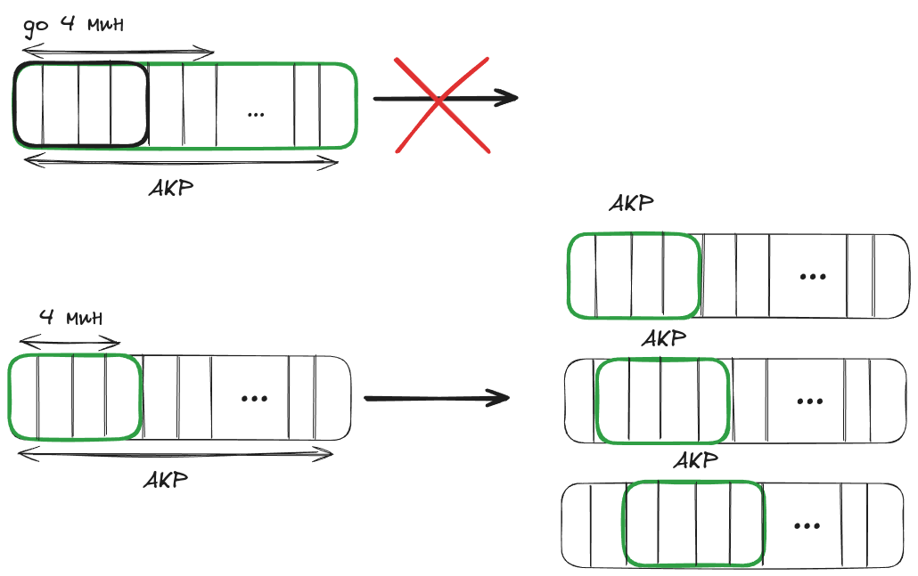
\includegraphics[width=1\textwidth]{pic/wind.png}
            \caption{Схематичное изображение примера применения скользящего окна к набору данных}
        \end{figure}

        Механизм преобразования интервалов данных с наличием и отсутствием АКР в
        блоки одинаковой длины с использованием скользящего окна заключается в
        последовательном выделении подмассивов фиксированной длины из исходного
        блока данных. Если длина блока превышает заданную целевую длину, из него
        формируются новые блоки путём ''скольжения'' окна фиксированной длины по
        исходному массиву данных. Начальная позиция окна сдвигается на
        определённое количество элементов (шаг скользящего окна) после каждого
        извлечения подмассива. Если же длина блока меньше целевой длины, то
        такой блок не используется при формировании нового набора данных.

        Например, если целевая длина блока равна \(n\), то первое окно
        захватывает элементы с 1-го по \(n\)-й, затем сдвигается на заданный шаг
        и захватывает элементы с \(2\)-го по \((n+1)\)-й и так далее, пока не
        будет достигнут конец исходного блока. Каждому выделенному подмассиву
        присваивается уникальный идентификатор, чтобы они рассматривались как
        отдельные новые блоки. Этот метод позволяет эффективно разбить исходные
        данные на множество частей одинаковой длины, сохраняя при этом локальную
        структуру данных и их временную последовательность.

        Для длины 4 получилась выборка в 18534 интервалов, для 16 - 17912
        интервалов, для 32 - 17280 интервалов. Затем для классических моделей
        машинного обучения осуществлялась балансировка количества элементов в
        обоих классах. Механизм балансировки выборок в рамках данной работы
        направлен на уравнивание количества блоков данных относительно классов,
        определяющих наличие или отсутствие АКР. Процесс начинается с разделения
        исходного набора данных на две подвыборки: одну, содержащую блоки с АКР,
        и другую, содержащую блоки без АКР. После этого определяется минимальное
        количество блоков между этими двумя группами. Если уже наблюдается
        равенство размеров групп, данные остаются неизменными. В противном
        случае, применяется метод ''undersampling'' к избыточной группе, то есть
        из неё случайным образом выбирается подмножество блоков, равное по
        размеру меньшей группе. Это достигается с использованием специального
        метода sample у объекта библиотеки Pandas, который случайным образом
        выбирает строки из группы, при этом фиксируется генератор случайных
        чисел через параметр random_state для обеспечения воспроизводимости
        результатов. Наконец, обе группы объединяются обратно в один набор
        данных, при этом количество блоков с наличием и отсутствием АКР
        становится одинаковым. Такой подход позволяет получить сбалансированный
        набор данных, который улучшает работу алгоритмов машинного обучения,
        особенно в случаях, когда дисбаланс классов мог бы привести к перекосу в
        сторону более многочисленного класса. Каждая из выборок была в
        дальнейшем разделена на подвыборки для обучения и для теста классических
        моделей МО (см. Таблица 2). Каждый из экспериментов проводился
        относительно блоков одной длины.

        \begin{table}[h]
            \centering
            \begin{tabular}{l|l|l|}
            \cline{2-3}
                                                & Обучающая выборка & Тестовая выборка \\ \hline
            \multicolumn{1}{|l|}{Блоки с АКР}   & 4512              & 1150             \\ \hline
            \multicolumn{1}{|l|}{Блоки без АКР} & 4547              & 1115             \\ \hline
            \end{tabular}
            \captionsetup{justification=centering}
            \caption{Информация о количестве блоках с АКР и без АКР в обучающей и тестовой выборках}
        \end{table}        

    \subsection{Параметры классических алгоритмов машинного обучения}

        Важно упомянуть, что относительно каждого временного ряда (т.е. для
        каждой частоты) создавалась отдельная модель машинного обучения, которая
        обучалась и тестировалась на данных своей определенной частоты. То есть
        процесс определения того, является ли приведенный интервал времени
        размерности 4, 16 или 32 блоком, в котором присутствует или отсутствует
        авроральное километровое радиоизлучение, состоял в следующем: для каждой
        частоты определенная модель прогнозировала класс, после чего выбиралось
        наиболее популярное значение класса среди всех моделей.
        
        Для обучения и тестирования моделей машинного обучения\\
        TimeSeriesForest, kNN и CatBoost были использованы следующие подходы.
        Модели TimeSeriesForest и kNN запускались с параметрами по умолчанию. В
        случае с TimeSeriesForest, алгоритм использует случайные подвыборки
        признаков для построения ансамбля деревьев решений, и по умолчанию
        используется количество деревьев, равное 500, а также другие параметры,
        такие как максимальная глубина деревьев и критерий расщепления,
        устанавливаемые внутренними значениями, оптимальными для большинства
        задач. Алгоритм kNN (k-Nearest Neighbors) использует стандартные
        параметры, такие как число соседей (по умолчанию 5) и метрику Евклида
        для расчета расстояния между точками, что делает модель простой, но
        эффективной для классификации в задачах с небольшими данными.

        Для модели CatBoost использовался подход с подбором гиперпараметров с
        помощью GridSearchCV. Для этого был определен список параметров с
        различными значениями для количества итераций (iterations), темпа
        обучения (learning_rate) и глубины деревьев (depth). Конкретно, для
        параметра iterations были протестированы значения от 1 до 5, для
        learning_rate — значения 0.01, 0.1 и 1, а для depth — значения от 1 до
        5. Использование GridSearchCV позволило найти оптимальные комбинации
        этих параметров и выбрать наилучшую модель CatBoost для предсказания.

    \subsection{Создание спектрограмм}    

        Затем, на основе выборок, полученных до балансировки, были созданы
        наборы данных для обучения алгоритмов компьютерного зрения (ResNet34,
        Xception, ViT), состоящие из спектрограмм. Отсутствие балансировки
        классов для ViT, ResNet и Xception обосновано спецификой работы данных
        моделей и характером задачи. Эти модели, основанные на глубоком
        обучении, обладают высокой способностью извлекать сложные паттерны из
        данных, что делает их менее чувствительными к дисбалансу классов по
        сравнению с более простыми алгоритмами. Во-первых, глубокие нейронные
        сети способны адаптироваться к дисбалансу классов за счёт использования
        взвешенных функций потерь. Например, при наличии дисбаланса можно
        назначать больший вес ошибкам на классе с меньшим количеством объектов,
        что позволяет компенсировать влияние преобладающего класса. Это
        устраняет необходимость прямой балансировки данных. Во-вторых, объём
        данных, используемый для обучения этих моделей, имеет достаточно
        элементов обоих классов для эффективного обучения. При этом модели
        обучаются учитывать соотношение между классами, представленное в данных,
        что делает выборку реалистичной и ближе к реальным условиям, в которых
        предполагается использовать модель. В-третьих, архитектуры ViT, ResNet и
        Xception обладают большой ёмкостью модели, что позволяет им изучать даже
        редкие шаблоны, характерные для уступающего в объеме образцов класса.
        Это контрастирует с алгоритмами меньшей сложности, которые могут быть
        склонны к переобучению на преобладающем классе, если дисбаланс не был
        устранён. Кроме того, в задачах, связанных с изображениями, балансировка
        данных может не всегда быть необходимой, так как модели могут извлекать
        важную информацию из структурных особенностей данных, независимо от их
        распределения. Таким образом, отсутствие балансировки позволяет моделям
        сохранять исходное распределение классов и лучше отражать реальные
        данные, что особенно важно при тестировании и развертывании модели.

        В данной работе для построения спектрограмм использовался алгоритм с
        использованием функции spectrogram из библиотеки scipy.signal.
        Спектрограммы строились для временных блоков данных с использованием
        различных параметров оконного преобразования в зависимости от длины
        блоков. Основной задачей было преобразовать временные ряды в набор
        спектральных изображений, пригодных для дальнейшего анализа.

        Для каждого блока, в зависимости от его длины, задавались определенные
        параметры оконного преобразования: длина окна и степень перекрытия между
        окнами. Для блоков длиной 4 использовалось окно длиной 2 с перекрытием
        1; для блоков длиной 16 — окно длиной 4 с перекрытием 2; для блоков
        длиной 32 — также окно длиной 4 с перекрытием 2. Эти параметры
        выбирались таким образом, чтобы обеспечить оптимальное разрешение
        спектра при сохранении информативности временных характеристик сигнала.

        Для каждого блока спектрограмма вычислялась отдельно для всех частотных
        каналов. Среднее значение спектральной мощности по всем каналам
        суммировалось и усреднялось для получения итоговой спектрограммы блока.
        Это позволило учесть вклад всех каналов и снизить влияние возможных
        шумов или выбросов в отдельных каналах. 

        Если итоговая спектрограмма имела крайне низкую мощность сигнала (что
        могло указывать на отсутствие полезной информации), она исключалась из
        дальнейшего анализа. Готовые спектрограммы визуализировались с помощью
        библиотеки Matplotlib в виде изображений, где оси времени и частоты были
        убраны для сохранения чистоты данных. Каждая спектрограмма сохранялась в
        виде изображения без полей, а информация о соответствующих блоках
        временного ряда и времени их начала сохранялась в виде структуры данных
        Pandas. Примеры изображений спектрограмм с учетом осей представлены
        ниже. Ось Y это нормализованные частоты (в долях от частоты
        дискретизации, при Частоте дискретизации равной 1 Гц). Ось X "---
        индексы временных окон (номера отсчётов). Временные метки $t$
        представляют центры временных окон. Каждая точка на оси X соответствует
        временному интервалу, в котором вычислялась спектральная плотность
        мощности. Центры временных окон "--- это моменты времени, которые
        соответствуют серединам каждого окна анализа в спектрограмме. Цветовая
        шкала определяет мощность спектра в логарифмическом масштабе (дБ).

        \begin{figure}[H]
            \centering
            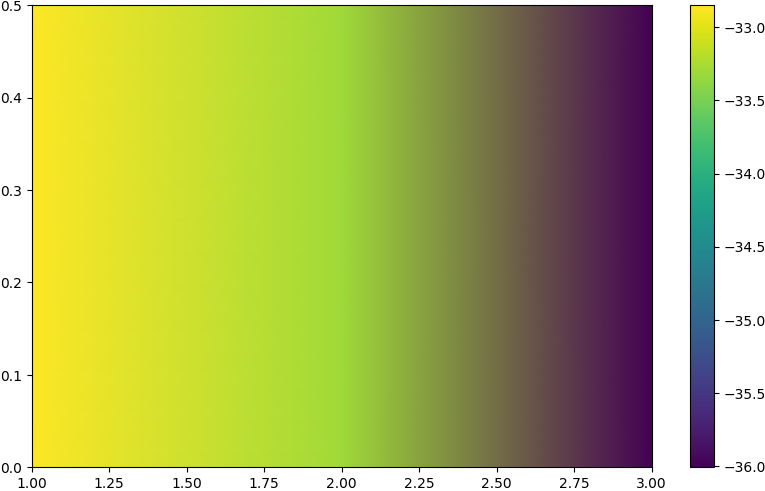
\includegraphics[width=0.7\textwidth]{pic/spect4.png}
            \caption{Пример спектрограммы, построенной на основе блока длиной 4}
        \end{figure}

        \begin{figure}[H]
            \centering
            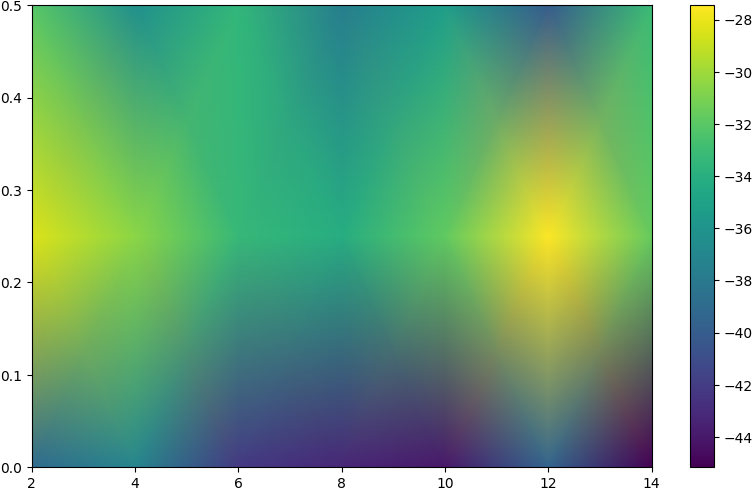
\includegraphics[width=0.7\textwidth]{pic/spect16.png}
            \caption{Пример спектрограммы, построенной на основе блока длиной 16}
        \end{figure}

        \begin{figure}[H]
            \centering
            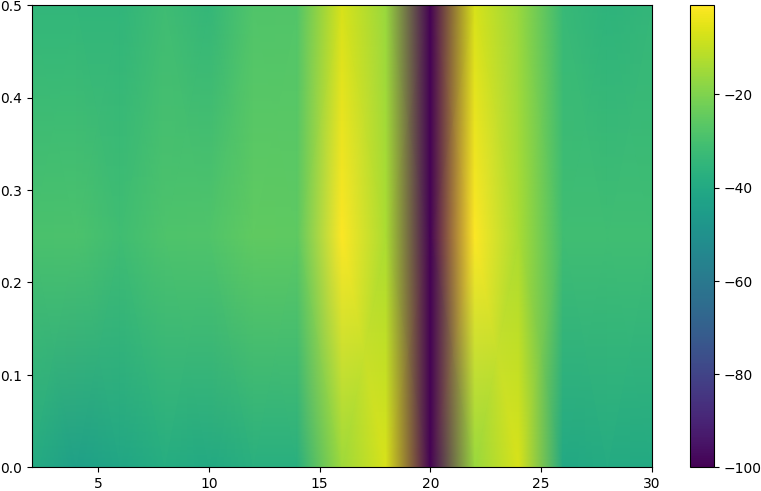
\includegraphics[width=0.7\textwidth]{pic/spect32.png}
            \caption{Пример спектрограммы, построенной на основе блока длиной 32}
        \end{figure}

        Подход обеспечил гибкость построения спектрограмм и возможность работы с
        временными рядами разной длины, создавая основу для дальнейшего
        применения спектральных изображений в рамках экспериментов. Информация
        про соотношение количества спектрограмм того или иного класса с длинами
        4, 16 и 32 содержится в таблице 3. Выборка изображений делилась на
        обучающую и тестовую в соотношении 4 к 1.

        \begin{table}[h]
            \centering
            \begin{tabular}{l|l|l|l|}
            \cline{2-4}
                                                              & Длина 4 & Длина 16 & Длина 32 \\ \hline
            \multicolumn{1}{|l|}{Кол-во спектрограмм с АКР}   & 5662    & 5345     & 5022     \\ \hline
            \multicolumn{1}{|l|}{Кол-во спектрограмм без АКР} & 12873   & 12567    & 12258    \\ \hline
            \end{tabular}
            \captionsetup{justification=centering}
            \caption{Количество спектрограмм с АКР и без АКР для блоков разной длины}
        \end{table}        

    \subsection{Параметры алгоритмов компьютерного зрения}
        
        Для обучения с последующей проверкой качества классификации спектрограмм
        каждая из моделей ViT, ResNet34 и Xception настраивалась с
        использованием соответствующих гиперпараметров и алгоритмов оптимизации.

        Для экспериментов с ViT использовалась предобученная архитектура
        google/vit-base-patch16-384, предоставляемая библиотекой transformers.
        Модель была модифицирована для задачи бинарной классификации с
        установкой параметра num_labels=2 и включением опции
        ignore_mismatched_sizes, которая позволяет корректно адаптировать
        размеры слоев к измененной задаче. В процессе обучения применялся
        оптимизатор AdamW с фиксированной скоростью обучения, равной \(5 \times
        10^{-5}\). Регулирование скорости обучения осуществлялось с помощью
        линейного планировщика (linear scheduler). Полный процесс обучения
        включал 5 эпох, что соответствует числу шагов обучения, равному
        произведению числа эпох и количества батчей в тренировочном наборе
        данных. 
        
        Для эксперимента с ResNet34 была использована архитектура ResNet34 с
        модификацией последнего полносвязного слоя. Вместо стандартного слоя был
        добавлен каскад из линейного слоя с 512 нейронами, функции активации
        ReLU, слоя дропаута с вероятностью 0.2, и финального линейного слоя с
        двумя выходами. Для расчета вероятностей классов использовалась функция
        LogSoftmax, обеспечивающая логарифмическую шкалу выходных вероятностей.
        В качестве функции потерь применялась отрицательная логарифмическая
        правдоподобность (NLLLoss), а оптимизация проводилась с использованием
        алгоритма Adam с коэффициентом скорости обучения \(1 \times 10^{-4}\).
        Процесс обучения включал 10 эпох, обеспечивающих достаточную сходимость
        параметров модели. 
        
        Модель Xception была реализована на основе предобученной версии,\\
        предоставляемой библиотекой timm. Архитектура адаптирована для задачи
        бинарной классификации. Для вычисления функции потерь использовалась
        отрицательная логарифмическая правдоподобность (NLLLoss), а оптимизация
        параметров осуществлялась алгоритмом Adam с фиксированной скоростью
        обучения \(1 \times 10^{-4}\). Обучение проводилось в течение 10 эпох,
        что обеспечивало стабильную производительность модели. 
        
        Все вычисления выполнялись с использованием графического процессора
        (GPU), что ускоряло процесс обработки данных и обеспечивало эффективное
        обучение моделей. Применение разнообразных архитектур, включая
        трансформерные и свёрточные нейронные сети, позволило провести
        сравнительный анализ их эффективности для задачи классификации
        спектрограмм, а также выявить преимущества и недостатки каждой из них.

    \subsection{Программная реализация}

        Перед обработкой данных было осуществлено преобразование исходных данных
        формата CDF в формат csv. Данный этап исследования содержится в файле
        ''preprocessing.py''. Этап обработки данных, балансирования выборок и
        разделения на обучающую и тестовую выборки для алгоритмов машинного
        обучения содержится в скрипте ''processing.py''. Процесс создания
        спектрограмм с последующим созданием набора данных для алгоритмов
        компьютерного зрения указан в файле ''spectrograms.py''. Процесс
        обучения и теста классических моделей машинного обучения содержится в
        ''classic.py''. Аналогично классическим моделям, для моделей
        компьютерного зрения программный код размещен в файле ''cv.py''.

    \subsection{Результаты}

        На основе проведенных экспериментов с алгоритмами машинного обучения, а
        также с алгоритмами компьютерного зрения, были получены результаты
        относительно каждой из выборок. Результаты представлены в Таблице 4. Все
        модели оценивались по трем основным метрикам: TPR (True Positive Rate),
        TNR (True Negative Rate) и F1-score. Метрика TPR, также известная как
        чувствительность, отражает долю правильно классифицированных
        положительных примеров среди всех положительных наблюдений, или же
        вероятность корректного определения блока с АКР в рамках конкретной
        выборки. Метрика TNR, также называемая специфичностью, измеряет долю
        правильно классифицированных отрицательных примеров среди всех
        отрицательных наблюдений, или же вероятность корректного определения
        блока без АКР в рамках конкретной выборки. F1-score, в свою очередь,
        представляет собой гармоническое среднее точности (Precision) и полноты
        (Recall), что делает его полезным для оценки моделей в условиях
        несбалансированных классов.

        \begin{table}[H]
            \centering
            \begin{tabular}{|c|c|c|c|c|c|c|}
            \hline
            Размер блока & Модель & TPR & TNR & F1-score \\ \hline
            4  & CatBoost & 0.00 & 1.00 & 0.00 \\ 
            4  & kNN & 0.74 & 0.90 & 0.80 \\ 
            4  & TimeSeriesForest & 0.75 & 0.89 & 0.80 \\ 
            4  & ViT & 0.30 & 0.90 & 0.76 \\ 
            4  & Xception & 0.91 & 0.30 & 0.70 \\ 
            4  & ResNet34 & 0.91 & 0.28 & 0.68 \\ \hline
            16 & CatBoost & 0.00 & 1.00 & 0.00 \\ 
            16 & kNN & 0.70 & 0.83 & 0.76 \\ 
            16 & TimeSeriesForest & 0.71 & 0.81 & 0.77 \\ 
            16 & ViT & 0.74 & 0.88 & 0.84 \\ 
            16 & Xception & 0.88 & 0.73 & 0.82 \\ 
            16 & ResNet34 & 0.66 & 0.84 & 0.77 \\ \hline
            32 & CatBoost & 0.00 & 1.00 & 0.00 \\ 
            32 & kNN & 0.69 & 0.80 & 0.75 \\ 
            32 & TimeSeriesForest & 0.70 & 0.79 & 0.76 \\ 
            32 & ViT & 0.97 & 0.99 & 0.98 \\ 
            32 & Xception & 0.97 & 0.98 & 0.97 \\ 
            32 & ResNet34 & 0.87 & 0.86 & 0.86 \\ \hline
            \end{tabular}
            \captionsetup{justification=centering}
            \caption{Значения метрик обучения моделей для различных размеров блоков}
        \end{table}
    
    На основании значений метрик также были построены графики зависимости
    значения каждой из метрик от длины блока (см. рисунки ниже).

    \begin{figure}[H]
        \centering
        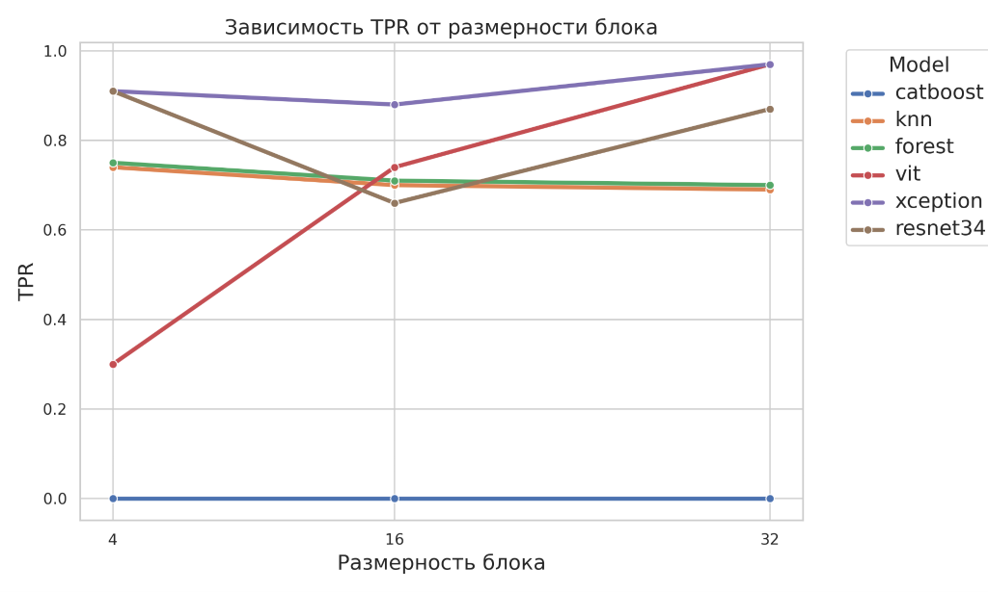
\includegraphics[width=1\textwidth]{pic/tpr.png}
        \caption{График зависимости метрики TPR от длины блока}
    \end{figure}

    \begin{figure}[H]
        \centering
        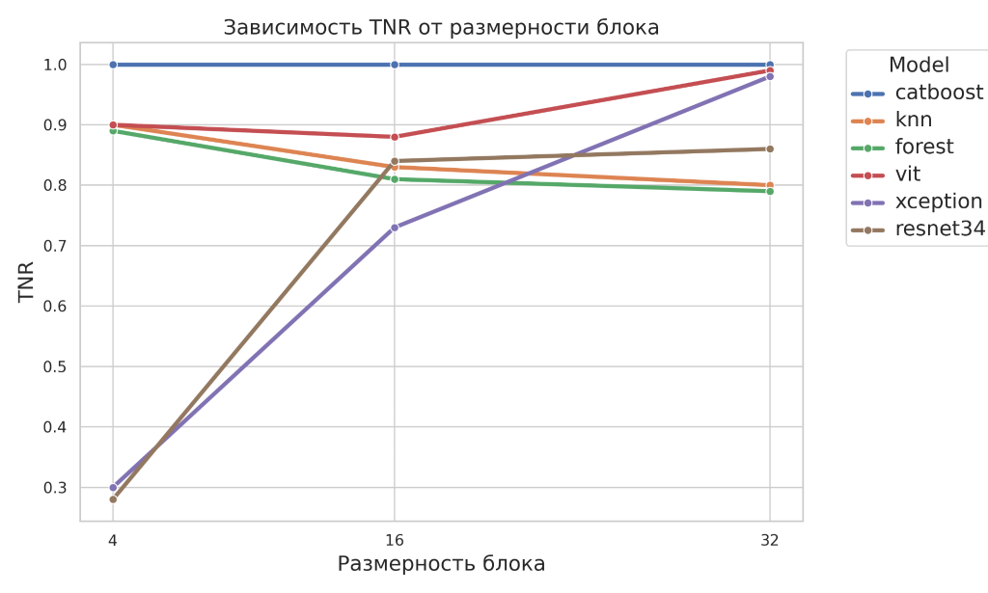
\includegraphics[width=1\textwidth]{pic/tnr.png}
        \caption{График зависимости метрики TNR от длины блока}
    \end{figure}

    \begin{figure}[H]
        \centering
        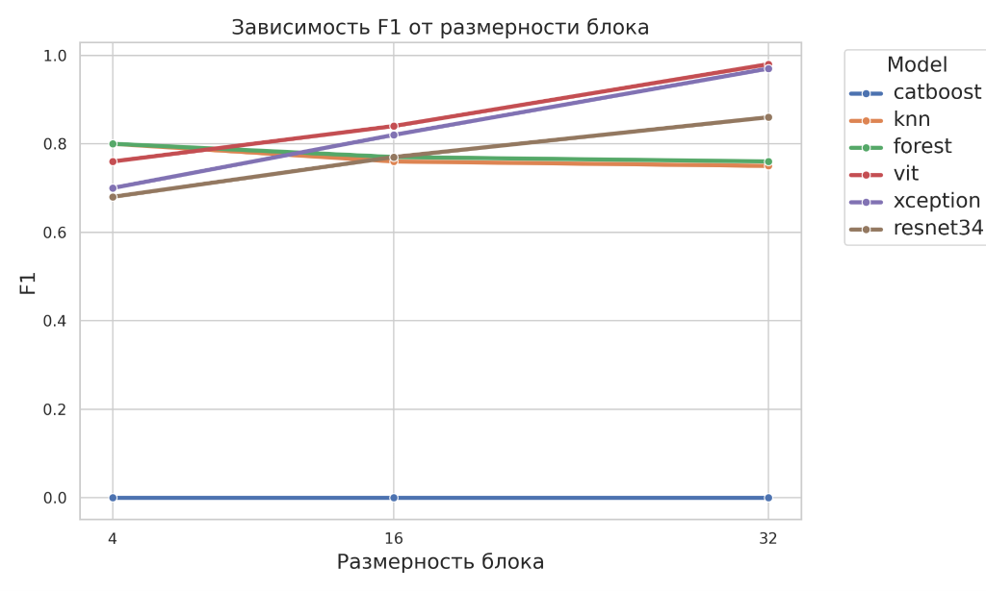
\includegraphics[width=1\textwidth]{pic/f1score.png}
        \caption{График зависимости метрики F1-score от длины блока}
    \end{figure}

\conclusion

    На основании полученных результатов можно отметить несколько ключевых
    выводов:
    
    \begin{enumerate}
        \item Предобработка данных при решении задачи существенно влияет на
        полученные результаты;
        \item Модели ViT и Xception демонстрируют наилучшие результаты при
        использовании блоков длиной 32, достигая значений F1-score 0.98 и 0.97
        соответственно;
        \item При увеличении размера блоков качество классификации всех
        алгоритмов компьютерного зрения растет;
        \item При увеличении размера блоков качество классификации всех
        алгоритмов классического машинного обучения, за исключением CatBoost,
        незначительно снижается;
        \item Модель CatBoost показала неспособность к успешной классификации,
        независимо от размера блоков, что может быть связано с её ограниченной
        способностью обрабатывать временные ряды в предложенной форме;
        \item Случайный лес и метод k ближайших соседей продемонстрировали
        приемлемую производительность (F1 Score = 0.8) на блоках длиной 4.
    \end{enumerate}

    Таким образом, выбор архитектуры модели и размера блока существенно влияет
    на процесс обнаружения аномалий (в рамках данного исследования в качестве
    аномальных данных мультивариативного временного ряда выступали интервалы, на
    которых наблюдалось авроральное километровое радиоизлучение). Также, в ходе
    экспериментов модели глубокого обучения, такие как ViT и Xception,
    продемонстрировали наиболее стабильную и высокую производительность. В
    дальнейшем следует изучить возможность применения более современных
    архитектур для решения задачи обнаружения аномалий с помощью классификации в
    мультивариативных временных рядах.


\begin{thebibliography}{99}
    % Введение

    \bibitem{unet} Zhang, Y. Human activity recognition based on time series
    analysis using U-Net / Y. Zhang, Z. Zhang, J. Bao, Y. Song // arXiv preprint
    arXiv:1809.08113. "--- 2018.

    \bibitem{anomalydetection} Schmidl, S. Anomaly detection in time series: a
    comprehensive evaluation / P. Wenig, T. Papenbrock // Proceedings of the
    VLDB Endowment. "--- 2022. "--- T. 15. "--- C. 1779-1797.

    \bibitem{anomalydetection2} Cheng, H. Detection and characterization of
    anomalies in multivariate time series / P. N. Tan, C. Potter, S. Klooster //
    Proceedings of the 2009 SIAM international conference on data mining. "---
    2009. "--- C. 413-424.

    % Временных ряды в задачах машинного обучения и их обработка

    \bibitem{tsnml} Gamboa, J. C. B. Deep learning for time-series analysis
    [Электронный ресурс] : [статья] / URL https://arxiv.org/pdf/1701.01887 (дата
    обращения 18.12.2024) Загл. с экрана. Яз. англ.

    \bibitem{fourier} Nussbaumer, H. J. The fast Fourier transform / H. J.
    Nussbaumer // Springer Berlin Heidelberg. "--- 1982. "--- C. 80-111.

    \bibitem{wavelet} Nason, G. P. Wavelet methods for time series analysis
    [Электронный ресурс] : [статья] / URL
    https://www.researchgate.net/publication/5068418_Wavelets_in_Time_Series_Analysis
    (дата обращения 18.12.2024) Загл. с экрана. Яз. англ.

    \bibitem{shapelet} Ye, L. Time Series Shapelets: A New Primitive for Data
    Mining [Электронный ресурс] : [статья] / URL https://
    www.cs.ucr.edu/\~eamonn/shaplet.pdf (дата обращения 18.12.2024) Загл. с
    экрана. Яз. англ.

    \bibitem{outliers} Tsay, R. S. Outliers in multivariate time series. / D.
    Pena, A. E. Pankratz // Biometrika. "--- 2000. "--- T. 87. "--- C. 789-804.

    \bibitem{spectrogram} Oppenheim, A. V. Speech spectrograms using the fast
    Fourier transform // IEEE spectrum. "--- 1970. "--- T. 7. "--- C. 57-62.

    \bibitem{spectrogram2} Nisar, S. An efficient adaptive window size selection
    method for improving spectrogram visualization. / O. U. Khan, M. Tariq //
    Computational intelligence and neuroscience. "--- 2016.

    \bibitem{stft} Mateo, C. Short-time Fourier transform with the window size
    fixed in the frequency domain. / J. A. Talavera // Digital Signal
    Processing. "--- 2018. "--- T. 77. "--- C. 13-21.
    
    \bibitem{stft2} Allen, J. Short term spectral analysis, synthesis, and
    modification by discrete Fourier transform. // IEEE transactions on
    acoustics, speech, and signal processing. "--- 1977. "--- T. 25. "--- C.
    235-238.

    \bibitem{tukey} Roy, T. K. Performance analysis of low pass FIR filters
    design using Kaiser, Gaussian and Tukey window function methods. / M.
    Morshed // In 2013 2nd international conference on advances in electrical
    engineering. "--- 2013. "--- C. 1-6.

    \bibitem{ddos} Borges, L. F. Multifaceted DDoS Attack Prediction by
    Multivariate Time Series and Ordinal Patterns [Электронный ресурс] :
    [статья] / URL
    https://www.researchgate.net/publication/382523397_Multifaceted_DDoS_Attack_Prediction_by_Multivariate_Time_Series_and_Ordinal_Patterns
    (дата обращения 18.12.2024) Загл. с экрана. Яз. англ.

    \bibitem{stfttcan} Tu, F. STFT-TCAN: A TCN-attention based multivariate
    time series anomaly detection architecture with time-frequency analysis for
    cyber-industrial systems [Электронный ресурс] : [статья] / URL
    https://www.sciencedirect.com/science/article/pii/S0167404824002669 (дата
    обращения 18.12.2024) Загл. с экрана. Яз. англ.

    \bibitem{forest} Liu, Y. New machine learning algorithm: Random forest. / Y.
    Wang, J. Zhang // In Information Computing and Applications: Third
    International Conference, ICICA 2012, Chengde, China, September 14-16. "---
    2012. "--- C. 246-252.

    \bibitem{catboost} Prokhorenkova, L. CatBoost: unbiased boosting with
    categorical features. / G. Gusev, A. Vorobev, A. V. Dorogush, A. Gulin //
    Advances in neural information processing systems. "--- 2018.

    \bibitem{knn} Guo, G. KNN model-based approach in classification. / H. Wang,
    D. Bell, Y. Bi, K. Greer // In On The Move to Meaningful Internet Systems
    2003: CoopIS, DOA, and ODBASE: OTM Confederated International Conferences,
    CoopIS, DOA, and ODBASE 2003, Catania, Sicily, Italy "--- 2003. "--- C.
    986-996.

    \bibitem{resnet} Zhuang, Q. Human-computer interaction based health
    diagnostics using ResNet34 for tongue image classification. / S. Gan, L.
    Zhang // Computer Methods and Programs in Biomedicine. "--- 2022. "--- T.
    226.

    \bibitem{xception} Wu, X. An xception based convolutional neural network for
    scene image classification with transfer learning / R. Liu, H. Yang, Z. Chen
    // In 2020 2nd international conference on information technology and
    computer application. "--- 2020. "--- C. 262-267.

    \bibitem{vit} Han, K. A survey on vision transformer. / Y. Wang, H. Chen, X.
    Chen, J. Guo, Z. Liu, D. Tao // IEEE transactions on pattern analysis and
    machine intelligence. "--- 2022. "--- T. 45. "--- C. 87-110.
    
    \bibitem{firstvit} Dosovitskiy, A. An image is worth 16x16 words:
    Transformers for image recognition at scale [Электронный ресурс] :
    [статья] / URL https://arxiv.org/pdf/2010.11929 (дата обращения 18.12.2024)
    Загл. с экрана. Яз. англ.

    % Метрики

    \bibitem{scores} Flach P. Performance evaluation in machine learning: the
    good, the bad, the ugly, and the way forward // Proceedings of the AAAI
    conference on artificial intelligence. – 2019. – Т. 33. – №. 01. – С.
    9808-9814.

    \bibitem{mat} Düntsch I. Confusion matrices and rough set data analysis / G.
    Gediga // Journal of Physics: Conference Series. – IOP Publishing, 2019. –
    Т. 1229. – №. 1. – С. 012055.

    \bibitem{space} Kurtz, M. J. The NASA astrophysics data system: Overview. /
    G. Eichhorn, A. Accomazzi, C. S. Grant, S. S. Murray, J. M. Watson //
    Astronomy and astrophysics supplement series. "--- 2000. "--- T. 143. "---
    C. 41-59.

    % Библиотеки

    \bibitem{python} DeVito, Z. Using Python for model inference in deep
    learning, [Электронный ресурс] : [статья] / URL https://
    arxiv.org/pdf/2104.00254.pdf (дата обращения 18.12.2024) Загл. с экрана. Яз.
    англ.

    \bibitem{fwpandas} Pandas [Электронный ресурс] : [сайт] / URL:
    https:// pandas.pydata.org/ (дата обращения 18.12.2024) Загл. с экрана. Яз.
    англ.

    \bibitem{fwspacepy} SpacePy [Электронный ресурс] : [сайт] / URL:
    https:// spacepy.github.io/ (дата обращения 18.12.2024) Загл. с экрана. Яз.
    англ.

    \bibitem{fwnumpy} NumPy. The fundamental package for scientific computing
    with Python [Электронный ресурс] : [сайт] / URL: https:// numpy.org/ (дата
    обращения 18.12.2024) Загл. с экрана. Яз. англ.

    \bibitem{fwsl} scikit-learn [Электронный ресурс] : [сайт] / URL:
    https:// scikit-learn.org/stable/ (дата обращения 18.12.2024) "--- Загл. с
    экрана.

    \bibitem{fwpyts} PyTS. A Python Package for Time Series Classification
    [Электронный ресурс] : [сайт] / URL: https:// pyts.readthedocs.io/en/stable/
    (дата обращения 18.12.2024) "--- Загл. с экрана.

    \bibitem{fwcatboost} CatBoost [Электронный ресурс] : [сайт] / URL:
    https:// catboost.ai/ (дата обращения 18.12.2024) "--- Загл. с экрана.

    \bibitem{fwpickle} pickle "--- Python object serialization [Электронный
    ресурс] : [сайт] / URL: https:// docs.python.org/3/library/pickle.html (дата
    обращения 18.12.2024) "--- Загл. с экрана.

    \bibitem{fwscipy} SciPy [Электронный ресурс] : [сайт] / URL:
    https:// scipy.org/ (дата обращения 18.12.2024) "--- Загл. с экрана.

    \bibitem{fwmatplotlib} Matplotlib: Visualization with Python
    [Электронный
    ресурс] : [сайт] / URL: https:// matplotlib.org/ (дата обращения 18.12.2024)
    "--- Загл. с экрана.

    \bibitem{fwseaborn} seaborn: statistical data visualization [Электронный
    ресурс] : [сайт] / URL: https:// seaborn.pydata.org/ (дата обращения
    18.12.2024) "--- Загл. с экрана.

    \bibitem{fwpytorch} PyTorch [Электронный ресурс] : [сайт] / URL:
    https:// pytorch.org/ (дата обращения 18.12.2024) Загл. с экрана. Яз. англ.

    \bibitem{fwtorchvision} torchvision [Электронный ресурс] : [сайт] / URL:
    https:// pytorch.org/vision/stable/index.html (дата обращения 18.12.2024)
    "--- Загл. с экрана.

    \bibitem{fwtimm} Pytorch Image Models (timm) [Электронный ресурс] :
    [сайт] /
    URL: https:// timm.fast.ai/ (дата обращения 18.12.2024) "--- Загл. с экрана.

    \bibitem{fwtransformers} Transformers [Электронный ресурс] : [сайт] /
    URL:
    https:// huggingface.co/docs/transformers/en/index (дата обращения
    18.12.2024) "--- Загл. с экрана.

\end{thebibliography}

\appendix

    \section{Листинг \texttt{preprocessing.py}}
    \inputminted{py}{code/preprocessing.py}

    \section{Листинг \texttt{processing.py}}
    \inputminted{py}{code/processing.py}

    \section{Листинг \texttt{spectrograms.py}}
    \inputminted{py}{code/spectrograms.py}

    \section{Листинг \texttt{classic.py}}
    \inputminted{py}{code/classic.py}

    \section{Листинг \texttt{cv.py}}
    \inputminted{py}{code/cv.py}


\end{document}
